\chapter{Results} \label{chapter-results}

% \epigraph{‘the map is not the territory’.}{Korzybski, A.  “A Non-Aristotelian System and its Necessity for Rigour in Mathematics and Physics”}
% % \epigraph{`In economics, models are spoken of as being made of physics when in truth they are made of Lego. They have that degree of provisionality and tentativeness and, importantly, rebuildability. There's a permanent invitation to take them apart and put them together again in a form that works better'}{John Lanchester \cite{lanchesterHowSpeakMoney2015}}
% \epigraph{ Models clarify the logic of hypotheses, ensure that predictions indeed follow from the premises, open our eyes to counterintuitive possibilities, suggest how predictions could be tested, and enable accumulation of knowledge.}{Peter Turchin \cite{turchinWhatEconomicsModels2017}}
% {\color{red} 

% % FIND EPIGRAPH

% CHECK ORDER - DO PARAMETER VALUES ASCEND OR DESCENT IN FIGURES - IN WHAT ORDER ARE THEY LISTED?}


The two main propositions of this thesis are, first, that financialization affects the ownership of housing and therefore the class structure of society, and, second, that this may have implications for urban productivity.  In this chapter, we present model results relevant to these propositions:  
% In this chapter we:
\begin{enumerate}
    \item % In the first part of this chapter, we 
    We describe the results from the model with no policy interventions. 
    \item We explore the effects of seven policy interventions in the model, % without the link from housing to productivity. In each case, 
    % For each intervention, we vary %show runs with two or more values of the policy 
    showing the effect of varying the parameters and discussing the effect of changes. 
    \item % In the third part, we 
    We then repeat the seven policy interventions, introducing a link from housing ownership to productivity, and comparing the revised model with the base case to explore how the productivity linkage affects the effectiveness of policy interventions. %With the link, increased rates of financialization affect productivity, reducing the pre-factor, $A$, in the scaling relationship. % 33\% % With the link, increased rates of financialized ownership reduce the value of the production parameter $A$. 
    % \item %In the fourth section, we
     % We next present the results with and without productivity impacts side-by-side to make it easier to and compare the effects of policies with and without the productivity linkage. 
     \item Finally, we explore the effects of a shock %Finally, section five illustrates the effect of a transitory policy shock 
     and demonstrate that the model exhibits \gls{hysteresis} or non-reversibility.
     
\end{enumerate}



\section{Seven policy interventions}

The policy variables we consider are: 

\begin{enumerate}
\item Capital gains taxes, which capture part or all of the speculative gains on property ownership.  A \gls{capital gains tax}  is a tax on the property price at the point of sale on the gains or profit accrued since the property was acquired. It captures the increase in the price of an asset due to changes in the market rather than any increase in value contributed by the owner. The Canadian capital gains tax rate is lower than the tax on interest or dividend income so capital gains are currently an especially attractive form of income for investors.
\item The cost of capital, or the rate at which investors can borrow, which affects the net return on property speculation.
\item Transportation costs, which are affected by public infrastructure investment, and reduce the amount of locational value that is spent on transportation, increasing the wealth of the community. 
\item Urban density, which is controlled by zoning regulation, and which multiplies locational rents. 
\item The sensitivity of the cost of borrowing to borrower wealth, which affects whether low-asset households can purchase housing and the likelihood they will service mortgages.
\item The property tax rate, which is a cost of living in the city. The tax is deducted from locational rents for individuals or speculators.
\end{enumerate}

Because there are multiple effects of each intervention, we use separate figures to represent the impact of each policy intervention on the trajectory of each of the seven indicator variables over time. %In the absence of linkages between the housing market and the production sector we see population effects but no effect on firm variables wage, capital stock or workforce. This is because we force the number of firms to accommodate increases in population. Different assumptions will allow growth in both firm size and number, but we are not interested in short-term firm dynamics, and the case we consider is easier to interpret. 

\section{Seven output variables}

The economic output variables we consider are wage, capital stock, firm workforce, total employment, city extent, number of firms and the share of properties owned by their occupants. 
% \begin{enumerate}
%     \item Wage levels
%     \item Capital stock
%     \item The size of the firm workforce
%     \item Total employment
%     \item City extent
%     \item Number of firms
%     \item The share of properties owned by their occupants.
% \end{enumerate} 
\begin{figure}[h!t]
\centering
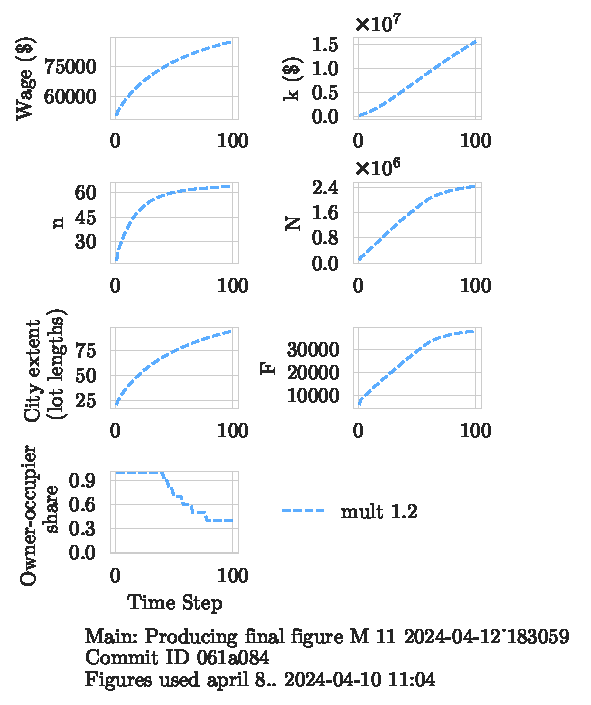
\includegraphics[scale=1.0, trim={0 1.4cm 0 0},clip]{fig/plain-for-intro_183059.pdf}
\caption[Graphic presentation of seven output variables]{Graphic presentation of seven output variables with baseline parameter settings. In the lower right the active parameter variations are indicated. In this case one parameter, `mult', is listed with its base value and with no variation.  `mult' stands for the `ratio of population affecting agglomeration,' indicating that the number of worker-residents is scaled up by 20\% to compose the population value.}
\label{fig:plain-for-intro}
\end{figure}
% We exhibit our results graphically.  
Figure~\ref{fig:plain-for-intro} shows the trajectory of each variable in the base model with no interventions. %Output for the baseline parameters of the model is illustrated in  % 
It is useful to describe the trajectory for each variable for the baseline case before we introduce the policy experiments.  
\begin{enumerate}
\item In the upper left is the equilibrium wage path.  Firms set a wage target based on the value of the marginal product of labour, which rises at a decreasing rate as the population rises due to the agglomeration effect on firm productivity.

\item The upper right shows the individual firm's capital stock $k$, which adjusts more slowly but rises as productivity and firm employment rise.  % Capital stock per worker is rising as we would expect.

\item Second from the top on the left, below the wage figure, is the number of workers in each firm, $n$. Firms set an employment target based on the value of the marginal product of labour, which rises due to the agglomeration effect. % The firm chooses 

\item On the right, below the capital plot, is the urban population $N$, which rises as the wage rises. There is circular causation between wage and population. Population increases feed back to increase the wage, a rising wage in turn drives population growth and population growth feeds back to productivity, increasing the wage. Rising transportation costs gradually slow growth. % This baseline case is for a small city that grows over one hundred years to have a population of approximately 2.4 million. 

\item In the third row, below the wage figure, is the city extent, which grows as the wage rises and homes are added to the periphery. 

\item To the right of the city extent is the number of firms $F$, which grows slightly slower than the population because firms increase their workforce size as productivity rises.

\item The final figure shows the share of properties owned by their occupants. The rest are owned as investment properties by speculators. This figure shows the effect of financialization when there is no feedback to productivity. 
% \item The key on the lower right labels experiment. In this case ``mult 1.2'' shows that the parameter that scales the labour force to population is 1.2, the standard setting. When a figure shows results for several parameter values different colours and line-styles are used for each.
\end{enumerate}


In total, there are forty-two plots in the first section, some showing a null effect. There are an additional forty-two plots in the second section. We discuss each experiment, point out the most significant effects, and provide some explanation of results that may seem surprising.  

\section{A note on how to interpret results}

Without strong empirical support for parameter values, we can say little about the magnitudes of any effects, although we can have some confidence in the directions and relative sizes.  
The results we present are conditioned on the selection of the parameters of the firm and migration models that form the environment for the housing market-financialization model. We have chosen parameter values to roughly approximate those for a mid-sized North American city so that the results may be more easily interpreted. The size of the effect we report would vary if different parameters had been chosen. % However the qualitative results are not affected by small variations in parameters. 
% It is important to remember that the results we report are qualitative, not quantitative results. 
%First we will explore the impact of financialization on productivity we will introduce explicit links between ownership and productivity in Chapter~\ref{chapter-tramsmission}
%We are currently observing these processes underway in the real world. We need to know if they are explained by a theoretically-consistent model of the urban economy that incorporates the financialization process.
For the experiments, we test relatively large perturbations of the parameters to make the effects of interventions clear. Appendix~\ref{appendix-parameters} documents the baseline parameter values. 

It is encouraging to note, given these constraints, that the results the model produces are consistent with theory, the stylized facts of urban development, and recent changes we are observing in cities. 
% We have two additional criteria in reviewing them. First, do the policy interventions we explore produce plausible results. Second, 
This suggests that the results may indeed provide insight into the effectiveness of the policy interventions we consider, and thus that these results might reasonably be used to suggest useful questions, hypotheses or topics for future work. 

%Since the purpose of this model is \gls{theoretical exposition}, the results are the results of explorations within the model and we make no claims about the outside world. % based on the results generated for the model. 

%The results are simply the output, given the relationships in the model. 
%

%We have built the model to allow us to investigate the effects of financialization on cities. work. % We've made the case that these questions matter given the process of financialization underway in cities. 


% We illustrate dramatic policy changes and strong productivity linkages to ensure the qualitative impacts are easy to identify. 




\section{The basic ownership result}

% Here's the trajectory of how the housing market is changing.

% Here's the result of the changes in ownership
% Here's what we see with the ownership pattern in the model.

% Summarize the process of financialization - not about a figure, what we're talking about in this picture.
% PLEASE SUMARIZE IT FIRST. 



% We are running the model and getting results about how the process we observe, build it into the model and see how the pattern of ownership changes, and we see the results of that. We see the changes in ownership based on this process running through the model.

% When we run the model with no parameter interventions, we see a steady rise in financialized ownership. 

%The model we've built is an attempt to build a theoretical model of a process like what we observe happening in the financialization of cities. 

The first question is whether the model produces the pattern % we observe happening in urban housing markets 
where investors own an increasing share of urban housing and home ownership is declining. % we have explained in previous chapters. 

\begin{figure}[h!tb]
\centering
\hspace{2cm}
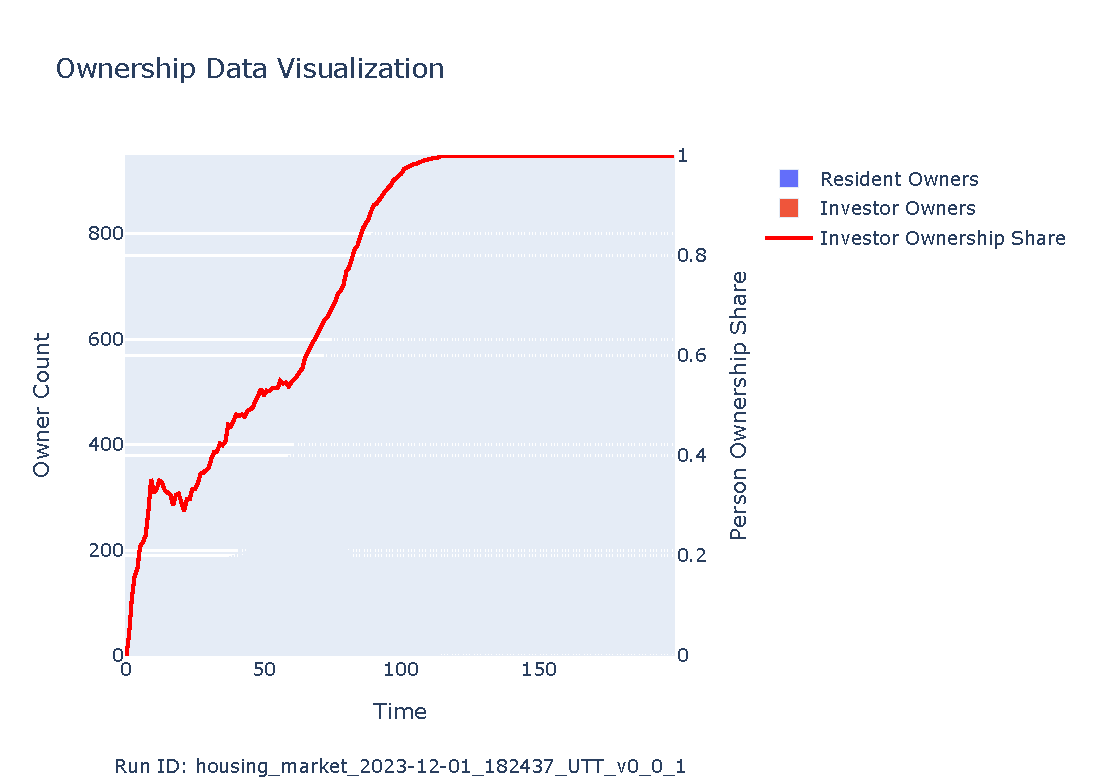
\includegraphics[scale=0.9, trim={0 1cm 0 1.8cm}, clip]{fig/Analysis/Ownership_Data_1.pdf}
\caption[The ownership result]{The transformation from a city of homeowners to a city of tenants in the baseline model.}
\label{fig:Baseline_ownership_trajectory}ti
\end{figure}


%Figure~\ref{fig:outcomes} summarizes a typical run of the model. 
Figure ~\ref{fig:Baseline_ownership_trajectory} illustrates the evolution of home ownership using a version of the model that grows over 200 years from 50 homeowners to a population of 1,000. The number of homeowners is shown by vertical blue bars.  Red bars show counts of investor-owners and the solid red line shows the share. This plot shows ownership numbers, while in the rest of this chapter, we report only shares. %The \gls{Alonso-Jacobs model} drives population. 
%Competition between would-be owner-occupiers and investors results in an evolving allocation of ownership of land. Within the model, properties are put up for sale, financial actors purchase an increasing number because they have advantages over private buyers. Primarily these advantages are related to increased ability to access capital and are based on realistic parameter values. The results are growing inequality, eviction and the loss of an urban class of homeowners, capturing and holding assets in the urban center. % The behaviours of the model agents combine to produce the results at the top of Figure~\ref{fig:outcomes}. 
% Before presenting the results, we briefly review how they arise and how the key ownership results are presented. 
The red line, with its scale on the right of the figure, shows the share of the housing stock owned by investors. 

At first, there are no investor-owned homes. %shown by red bars.
The number of owner-occupiers initially rises faster than the number of investors, but after one hundred periods it falls to zero. By the time the city reaches its maximum size, the city has transformed from a city of homeowners to a city of tenants. The unevenness in the rise of the red line signals a transitional range in which investors and would-be owner-occupiers are similar in number and competitive in strength. In that range, randomness in the savings of new entrants affects the number of units going to each type of buyer. 

Investors eventually own all of the housing in this example.  With plausible parameter settings, our model consistently produces trajectories similar to this example. This result supports the hypothesis that without countervailing forces, financial actors will take an increasing share of ownership in the housing market. The tendency for investors to own an increasing share of the housing stock is robust across experiments in the model. 
 %\footnote{Recall that the radius of a circular city is proportional to the wage premium. Rent can be visualized as a cone of volume $\pi r^2 h/3$ where $h$ is the wage premium. If we double $h$, the volume is increased by a factor of 8.}




%The pattern of ownership established this way determines how locational rents within the city are distributed. %The consequences of any shift from owner-occupancy to tenancy, shown in red, are dramatic. 
%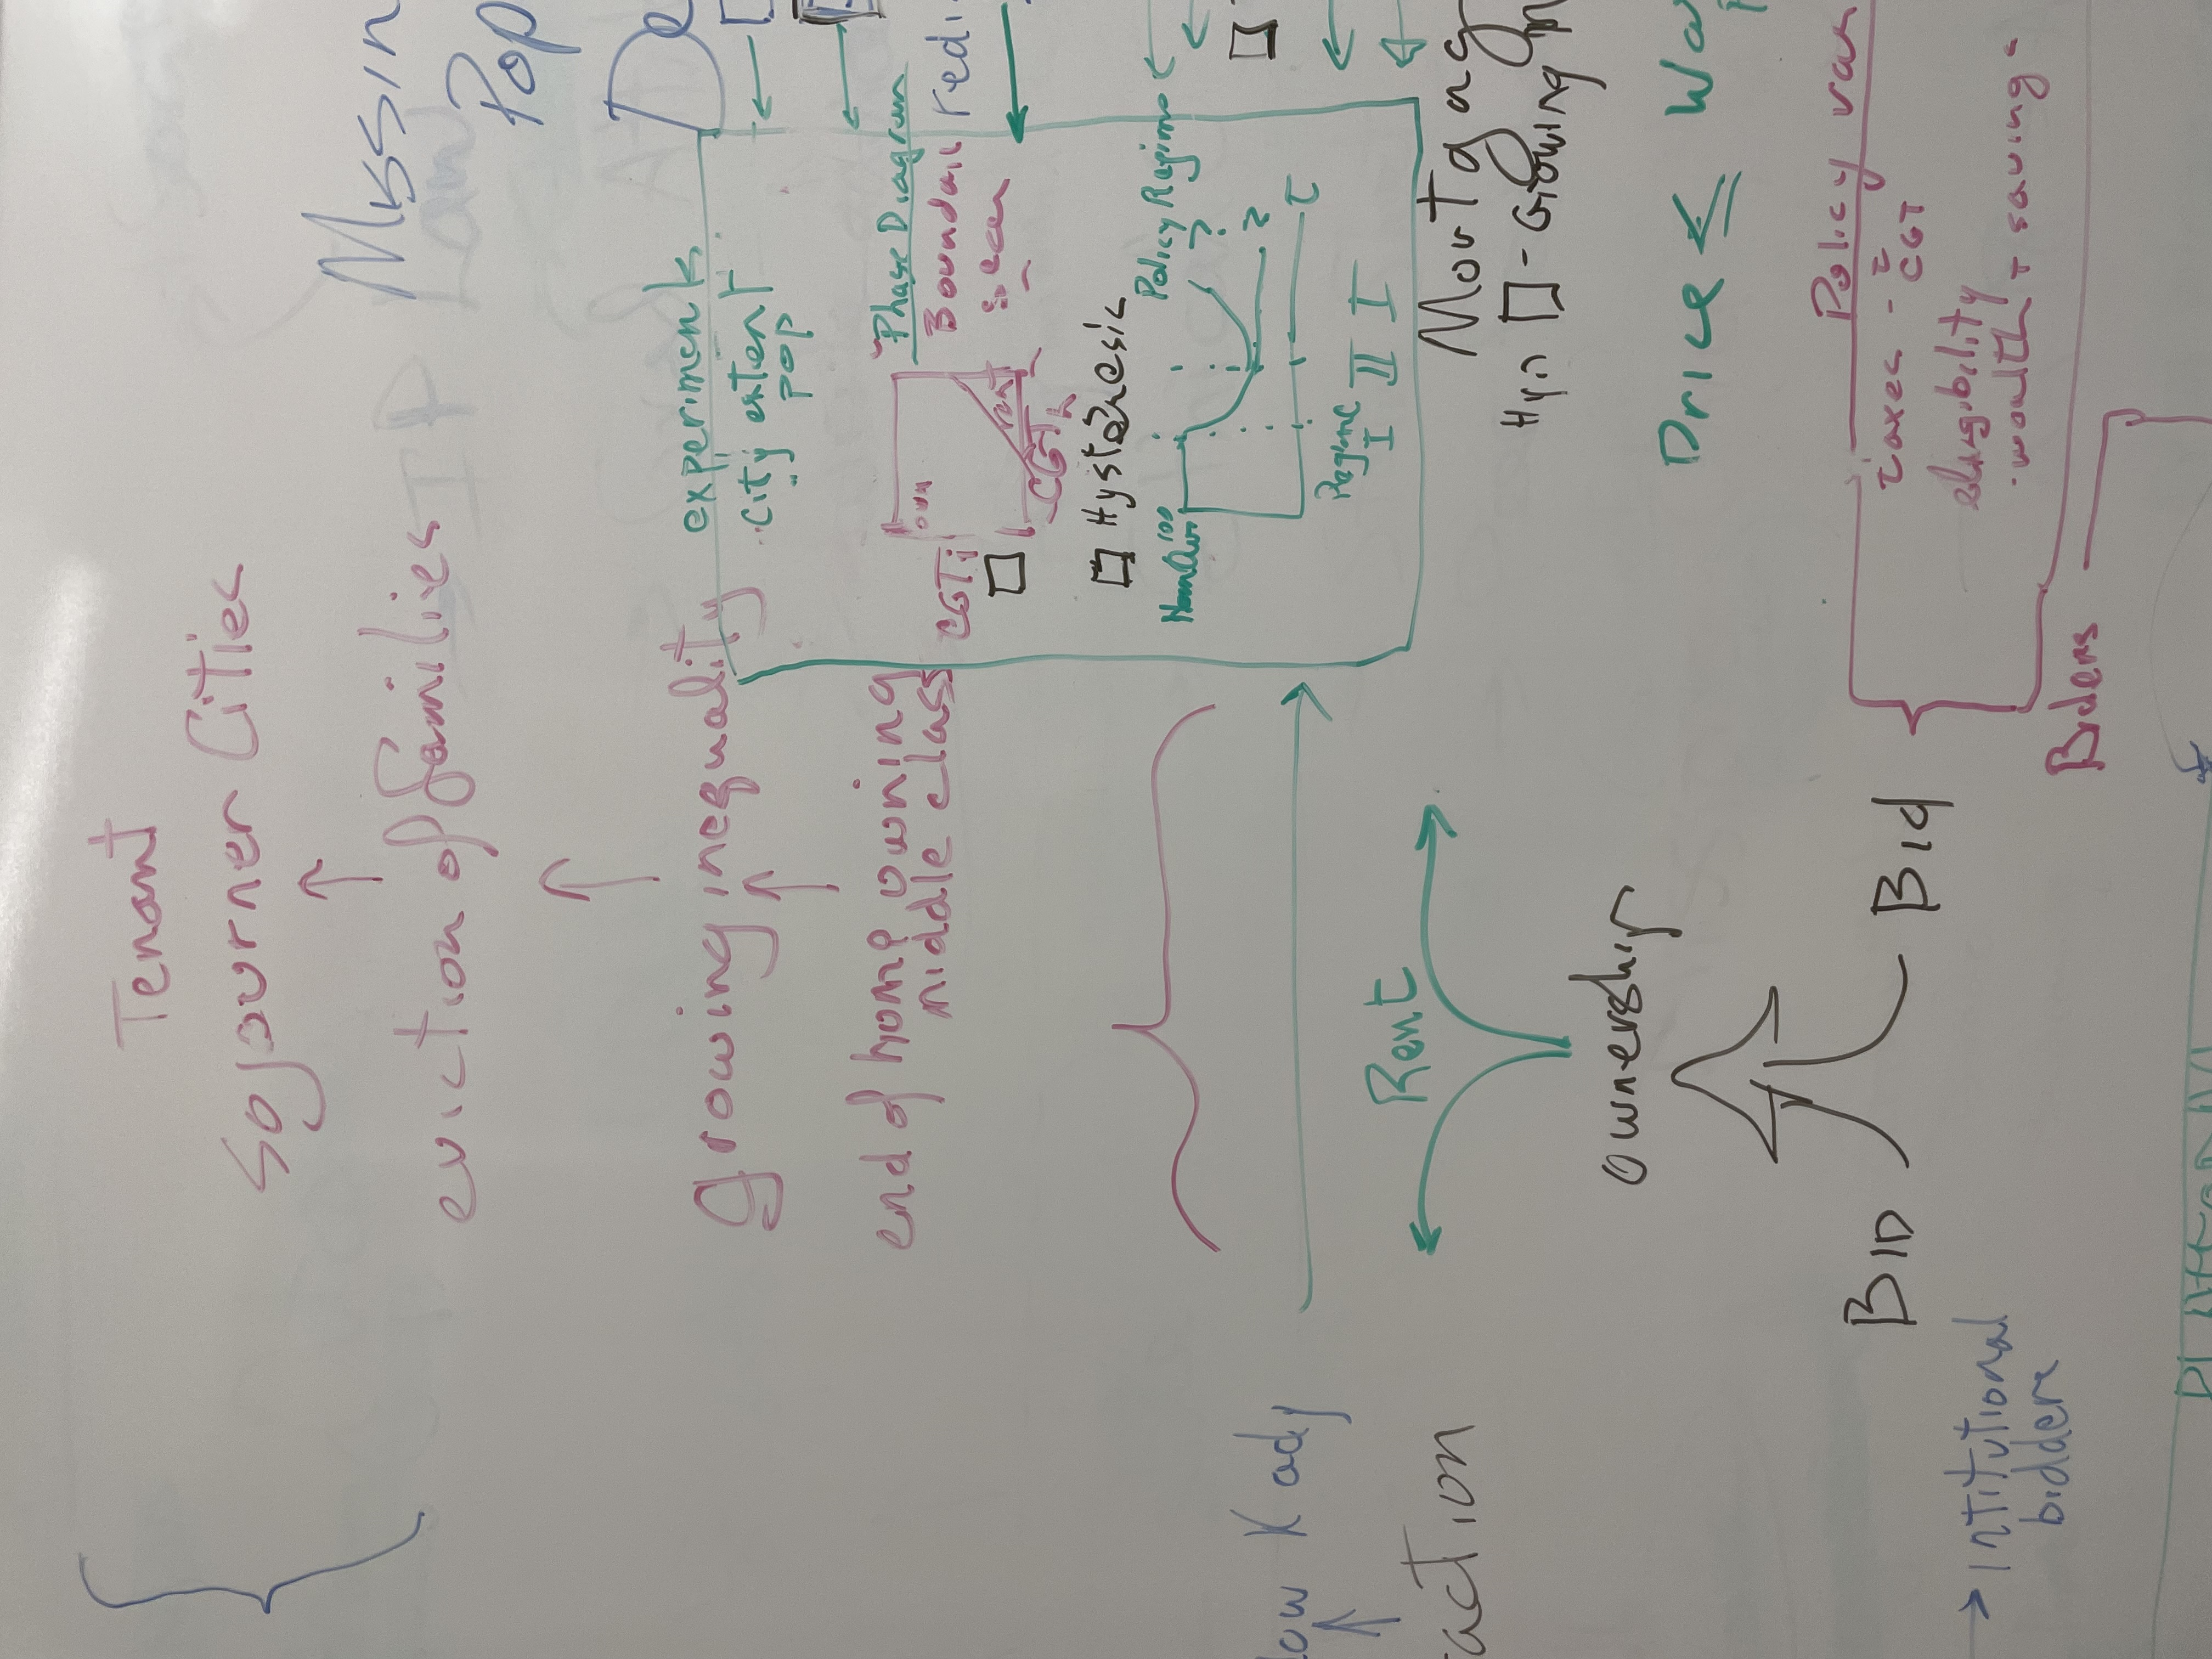
\includegraphics[scale=.5, angle=-90]{fig/IMG_2691.jpg}
The distribution of ownership determines the distribution of the locational land rents, which are the product of agglomeration effects, so this example sees owners of capital capturing an increasing share of the surplus value generated by urban agglomeration. %Initially, 100\% of locational land rent accrues to residents.   
As the city grows, rents increase. Total annual locational rents a hundred steps in, at the end of the run, are approximately twenty times their initial size. At that point, 100\% of the surplus accrues to the owners of financial capital.

% \hspace{1.5cm}

% \newpage
\section{Policy interventions without the productivity link}

This section examines the seven potential policy interventions, introduced above, and their effects over 100 periods on city size, wage level, and home ownership. In each case, we vary one parameter to simulate a policy  intervention, % that can be determined  or influenced by public policy 
and examine the effect on the city's evolution.

\subsection{Capital gains tax on investors}
A \gls{capital gains} tax is a tax on profit from the sale of property or an investment. It captures the increase in the price of an asset due to changes in the market rather than any increase in value contributed by the owner.\footnote{The Canadian capital gains tax rate is lower than the tax on interest or dividend income so capital gains are an especially attractive form of income for investors. In Canada, homeowners currently do not pay capital gains taxes on their primary residence. % This is a policy that has been questioned because it favours owners over renters whose investments would be subject to taxes. 
} We define any homeowner who does not occupy the housing unit they own as an investor. 
\begin{figure}[!hbtp]
\centering
% \raggedleft
% \hspace{5cm}
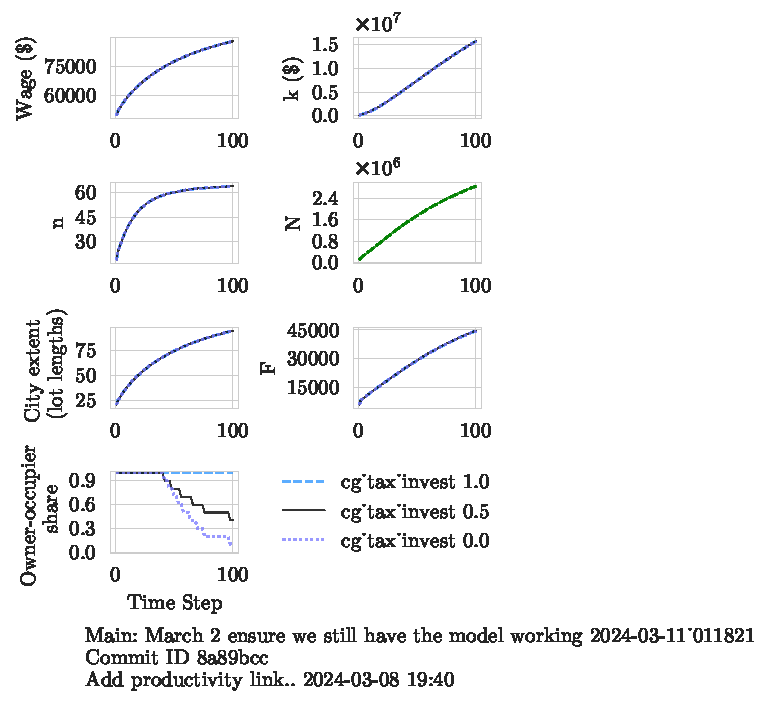
\includegraphics[scale=0.9, trim={0 1.4cm 4cm 0},clip]{fig/cg_tax_invest-Main-011821.pdf}
\caption[The effect of changing the capital gains tax for investors]{The effect of changing the capital gains tax for investors. This figure illustrates the effect on seven policy variables over time, with a capital gains tax rate of 0\%, 50\%, and 100\% for investors, the default 1\% rate for homeowners, and no productivity linkage.}
\label{fig:CGinvest_ownership_trajectory}
\end{figure}
The baseline value for the capital gains tax is 15\% for investors and 1\% for owner-occupiers, who are exempt from capital gains tax on their first residence, but have some costs to realize their capital gains. In this experiment, we explore the effect of substantial changes to the capital gains tax rate for investors. 
We substitute three levels of capital gains tax for investors (0\%, 50\%, and 100\%), keeping the tax level constant at 1\% for homeowners.

In general, since capital gains are part of the objective of investors, a capital gains tax should, in theory, reduce investor participation. Figure~\ref{fig:CGinvest_ownership_trajectory} shows that if 100\% of gains are taxed away, investors do not enter the market. A capital gains tax on housing investment will have a powerful effect on the ownership ratio. It does not, however, affect the other economic variables. % The result was achieved in a situation where homeowners pay a capital gains tax of 1\%  when they sell. 

\newpage
\subsection{Capital gains tax on owner-occupiers}
We can also change the capital gains tax for homeowners. 
Figure ~\ref{fig:CGpers_ownership_trajectory} shows of the effect of four different capital gains tax rates, 0\%, 10\%, 20\% and 30\% on owner-occupiers. The capital gains tax rate for investors in this set of experiments is 15\%. Increasing the capital gains for owners makes purchasing a home less attractive as an investment for owner-occupiers but not for non-resident owners. %Rents do not fall for tenants in our mode, however. Landlords continue to charge tenants the full locational value and the locational value does not depend on whether there are capital gains for property owners. 


There's a bifurcation in the ownership results depending on whether the rate is above or below the investor's tax rate.  If the owner-occupiers' tax rate is higher than the rate for investors,  shown by the solid and the dashed lines,  the homeownership rate is  30\% lower at 100 time steps. 

% {\color{red} MAKE THIS MORE CLEAR - What if VALUE IS THE SAME. }

\begin{figure}[h!t]
\centering
% \raggedleft
% \hspace{5cm}
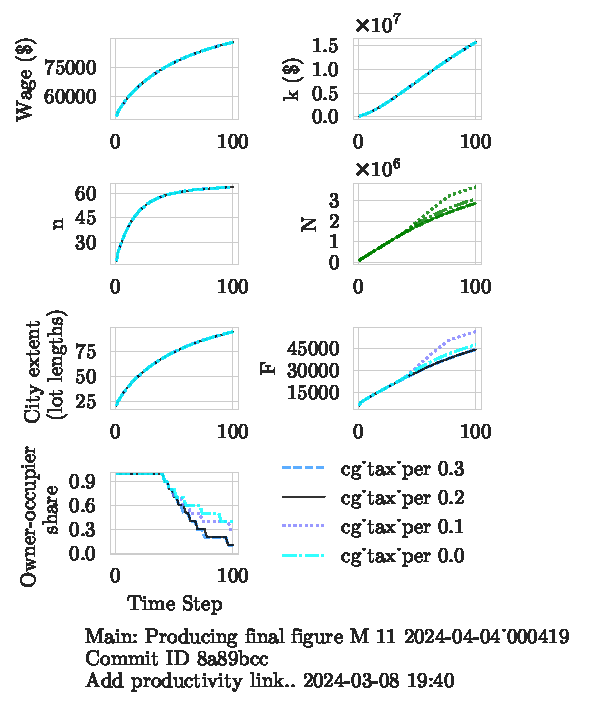
\includegraphics[scale=0.9, trim={0 1.4cm 0 0},clip]{fig/cg_tax_per-000419.pdf}
\caption[The effect of introducing a capital gains tax for owner-occupiers]{The effect of introducing a capital gains tax for owner-occupiers. This figure illustrates the effect on seven policy variables over time, with a capital gains tax rate of 0\%, 10\%, 20\% and 30\% for owner-occupiers, the default 15\% rate for investors, and no productivity linkage.}
\label{fig:CGpers_ownership_trajectory}
\end{figure}


%%%%%%%%%%%%%
\newpage

\subsection{The cost of capital for investors}
% {\color{red} DO WE WANT TO TRY LARGER RANGE -- No. there is more interest in finer divisions around 0.15 }
% 'r_investor': [0.2, 0.1, .05] has set up for morning
The cost of capital is the interest rate on borrowed money. Higher capital costs for investors might be expected to slow the rate of housing acquisition because it makes acquiring housing more expensive for investors. Figure ~\ref{fig:capital_ownership_trajectory} shows that increasing capital costs for investors does not affect the final level of investor ownership.  It does, however, decrease the wage slightly and, therefore, decrease the population. This suggests that the model appears to be less sensitive to the cost of money, than to other interventions. % The cost of capital for investors is therefore not an obvious policy tool in the urban context.

\begin{figure}[h!t]
% \centering
\raggedleft
\hspace{5cm}
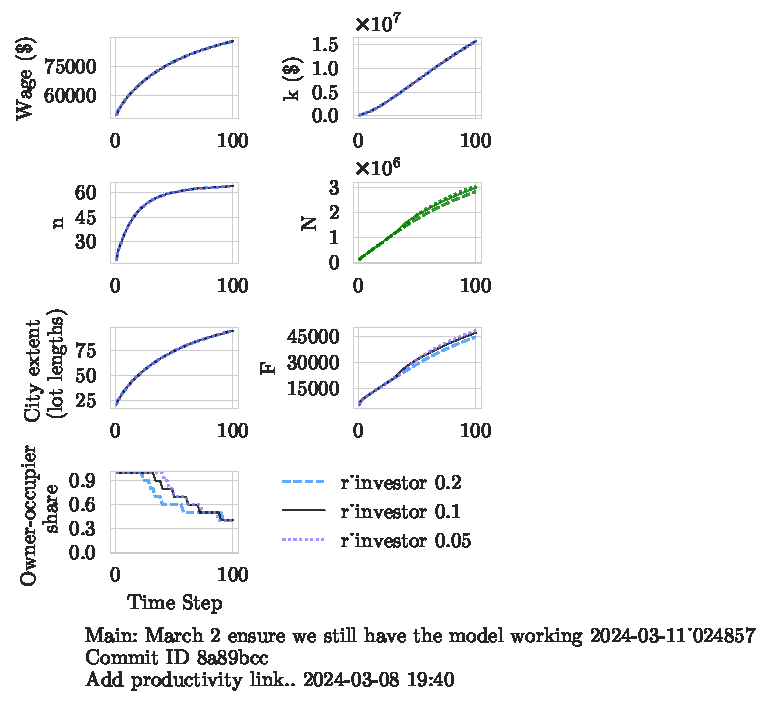
\includegraphics[scale=0.9, trim={0 1.4cm 0 0},clip]{fig/r_investor-Main-024857.pdf}
\caption[The effect of raising capital costs for investors]{The effect of raising capital costs for investors. This figure illustrates the effect on seven policy variables over time, with an investor rate of 5\%, 10\% and 20\%, a rate for owner-occupiers near 5.1\%, just above the bank's prime rate, adjusted based on individual assets and income, and no productivity linkage.}
\label{fig:capital_ownership_trajectory}
\end{figure}

\newpage

\subsection{Transportation costs} 
Transportation costs are the costs of getting from a residence to work. Policy can shape transportation costs through, for instance, improving roads, managing road congestion, or supplying public transit. % Can reducing the cost of transportation affect the ownership ratio? 
Figure~\ref{fig:c_ownership_trajectory}, shows the results of reducing transportation costs for all residents by 40\%. 
%This is what we expect in the Alonzo model within this model.
The city grows faster and gets larger with lower transportation costs. % and this effect is, indeed, observed, as expected. %We expect the city would 
% 'c': [500, 300],

%{\color{red} HOW DO WE EXPLAIN THE EFFECT OF TRANSPORTATION ON THE OWNERSHIP SHARE?}

\begin{figure}[h!b]
\centering
% \raggedleft
% \hspace{5cm}
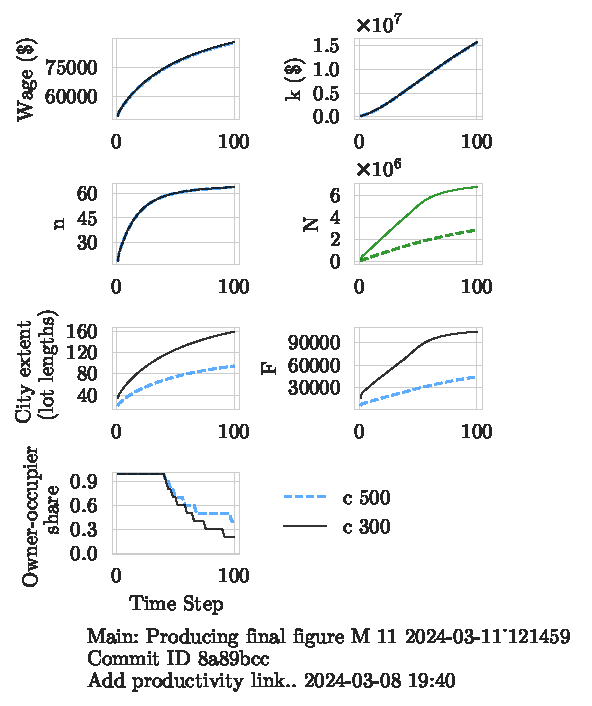
\includegraphics[scale=0.9, trim={0 1.4cm 0 0},clip]{fig/c-Main-121459.pdf}
\caption[The effect of decreasing transportation costs]{The effect of decreasing transportation costs. Illustrates the effect on seven policy variables over time, with a cost of \$300 and \$500 per unit distance per year, and no productivity linkage.}
\label{fig:c_ownership_trajectory}
\end{figure}


Surprisingly, lower transportation costs also served to decrease the home-ownership ratio. This is likely because the reduction in transportation costs leads to an increase in willingness to pay land rents. The resulting increase in land rents allows prices to rise, leading to higher expected capital gains.  Investing in housing is then more attractive for speculators and increased participation by speculators leads to less ownership by residents. 

%A slight decrease in the wage can be seen. 


\newpage


\subsection{Density}
% 'density': [100, 150]
% Density is a policy variable that is much discussed. 
Density is the number of residents per grid space. Increasing density is proposed as a way to increase the availability of housing and the ability of people to buy homes. Figure~\ref{fig:density_ownership_trajectory} shows that the effect of density on city population is significant. It has no effect, however, on the city's extent, and no effect on the ownership ratio.


\begin{figure}[h!bt]
\centering
% \raggedleft
% \hspace{5cm}
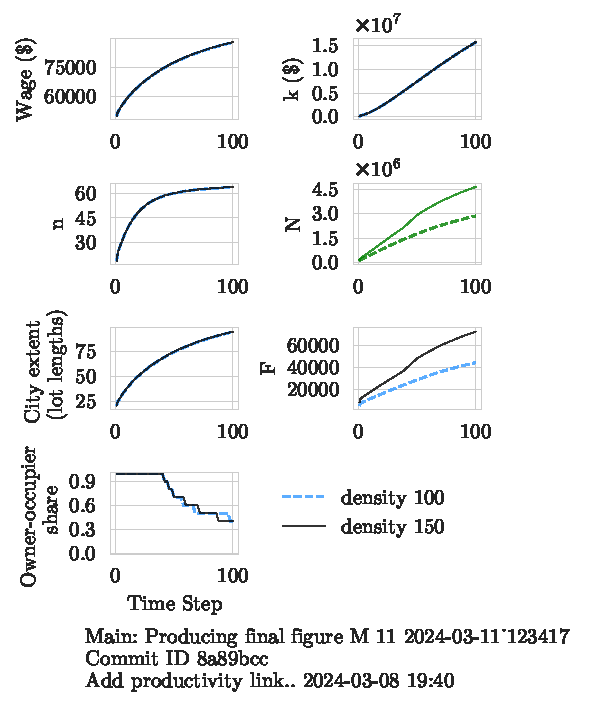
\includegraphics[scale=0.9, trim={0 1.4cm 0 0},clip]{fig/density-Main-123417.pdf}
\caption[The effect of increasing density]{The effect of increasing density. This figure illustrates the effect on seven policy variables over time, with a population density of 100 and 150 per grid space, and no productivity linkage.}
\label{fig:density_ownership_trajectory}
\end{figure}

Increasing density does not affect long-term ownership ratios because rent per unit is unchanged, so density alone does not affect the relative advantage of new home buyers. % and investors, leaving the ratio constant. 
%  the share of homeowners is not affected, only the number of homes is. 
There are more homes, however, and since the ratios are consistent, there are more homeowners overall. % This result may be fragile. {\color{red} WHY}

\newpage

% \subsection{Wealth requirements for new home buyers}
\subsection{Cost of financing's dependence on borrower's wealth}
% Cost of financing's dependence on borrower's wealth

Wealth sensitivity % is a parameter of the banking system. It that 
determines the assets required for people to secure a mortgage. A higher parameter value is more restrictive. Figure~\ref{fig:Wealth-based} in Chapter~\ref{chapter-model} on the model illustrates the effect of the parameter on the maximum mortgage available to borrowers with different asset levels. % ,  making it more harder for those with fewer assets to get a mortgage.
% {\color{red} CLARIFY - THIS DOES NOT MAKE CLEAR IF IT RAISES THE THRESHOLD OR RAISES THE COST}

\begin{figure}[h!bt]
\centering
% \raggedleft
% \hspace{5cm}
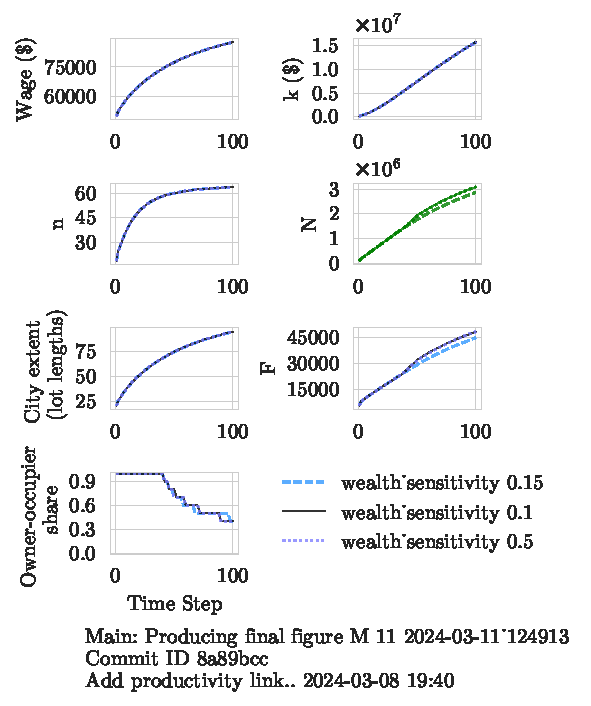
\includegraphics[scale=0.9, trim={0 1.4cm 0 0},clip]{fig/wealth_sensitivity-124913.pdf}
\caption[The effect of the wealth sensitivity parameter]{The effect of the wealth sensitivity parameter. This figure illustrates the effect of the parameter on seven policy variables over time, with parameter values of 0.15, 0.1, and 0.5, and no productivity linkage. The wealth sensitivity parameter controls the wealth required for accessing a mortgage and its effect is illustrated in Figure~\ref{fig:Wealth-based} in the model chapter.}  
\label{fig:wealth_sensitivity_ownership_trajectory}
\end{figure}

Figure~\ref{fig:wealth_sensitivity_ownership_trajectory} illustrates that a restrictive mortgage regime slightly reduces the labour supply and city population. It has no noticeable effect on the ownership ratio. % Since the purpose of a restrictive policy is to reduce defaults and bankruptcies, the small impact on other variables suggests that as a policy it can be adopted without needing to consider the economic impacts on the city. 
% 'wealth_sensitivity': [0.15, 0.1, 0.5]
% {\color{red} DISCUS WHY IT MIGHT HAVE NO IMPACT ON CITY POPULATION}

\newpage



\subsection{The property tax rate}

The property tax rate is the annual tax paid, as a share of the property's total value. We consider a property tax rate between 1\% and 10\%.
% 'property_tax_rate': [0.1, 0.05, .01] k doing}
\begin{figure}[h!b]
\centering
% \raggedleft
% \hspace{2cm}
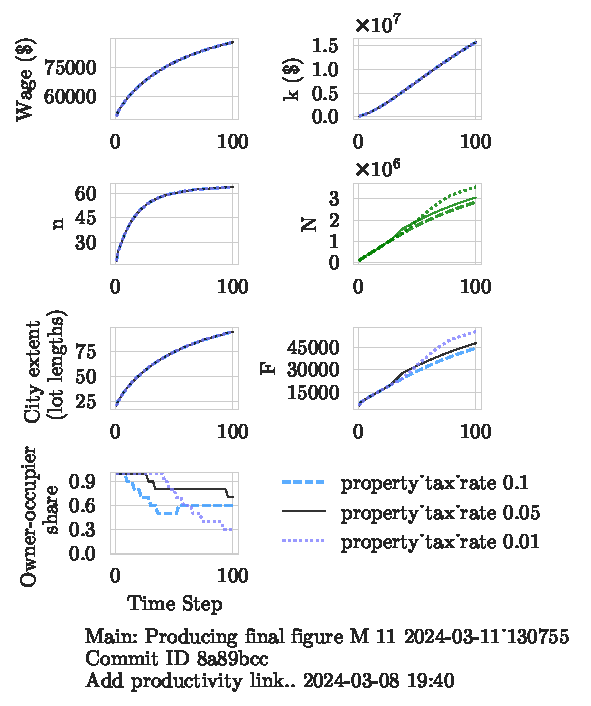
\includegraphics[scale=0.9, trim={0 1.4cm 0 0},clip]{fig/property_tax_rate-Main-130755.pdf}
%{fig/property_tax_with_5_202807.pdf}
\caption[The effect of varying the property tax rate]{The effect of varying the property tax rate. Illustrates the effect on seven policy variables over time, with rates between 1\% and 10\%, and no productivity linkage.}
\label{fig:property_tax_ownership_trajectory}
\end{figure}
Figure~\ref{fig:property_tax_ownership_trajectory} shows that the effect of the property tax varies with the size of the tax. The highest rate we consider decreases city size as shown by the dashed blue line. % A cluster of slightly lower values raise population but make no difference to the ownership ratio. 
% A very low value of 1\%, shown in red, appears to slow growth initially then increases it. Interestingly, this very low rate results in a higher degree of financialization of the housing stock. % Two effects may explain this result. 
% First, a higher growth rate makes housing a more attractive investment and second low property taxes reduce the operating costs of rental properties.
A higher property tax rate reduces the share of the locational rent captured by investors. % This % The effect is analogous to increasing the capital gains tax for property investors, as discussed in subsection~\ref{subsec:CGinvest}.
It does seem to affect the ownership ratio. The results suggest that departure from the current level in either direction might lead to a greater decline in the fraction of owner-occupiers. Further analysis would be required to more fully characterize this result.


% {\color{red} DISCUSS - THIS LOOKS LIKE A BIFURCATION - SOME THRESHOLD WHERE IT AFFECTS LEVELS.. - CAN WE CHARACTERIZE IT? SEVERAL MORE VERY LOW RATES, SEVERAL MUCH HIGHER RATES..Could we try 0\% and/or some exploration around the lower level?}

% {\color{red} trying moving this. MAYBE THIS IS PART OF A DISCUSSION here }
% The property tax rate is a matter for policy debate because there are good reasons to think, first, that property taxes are a barrier to ownership, and second, that the property taxes are not paying all the costs of public infrastructure and services to homeowners, leading to significant inequities. The implications of this result are..


% {\newpage\thispagestyle{empty}
% \vspace{-1.5cm}
\begin{figure}[h!tb]\label{fig-impact-channels2}
%\vspace{-1cm}
\begin{adjustwidth}{-0.24\textwidth}{-0.24\textwidth}
\centering
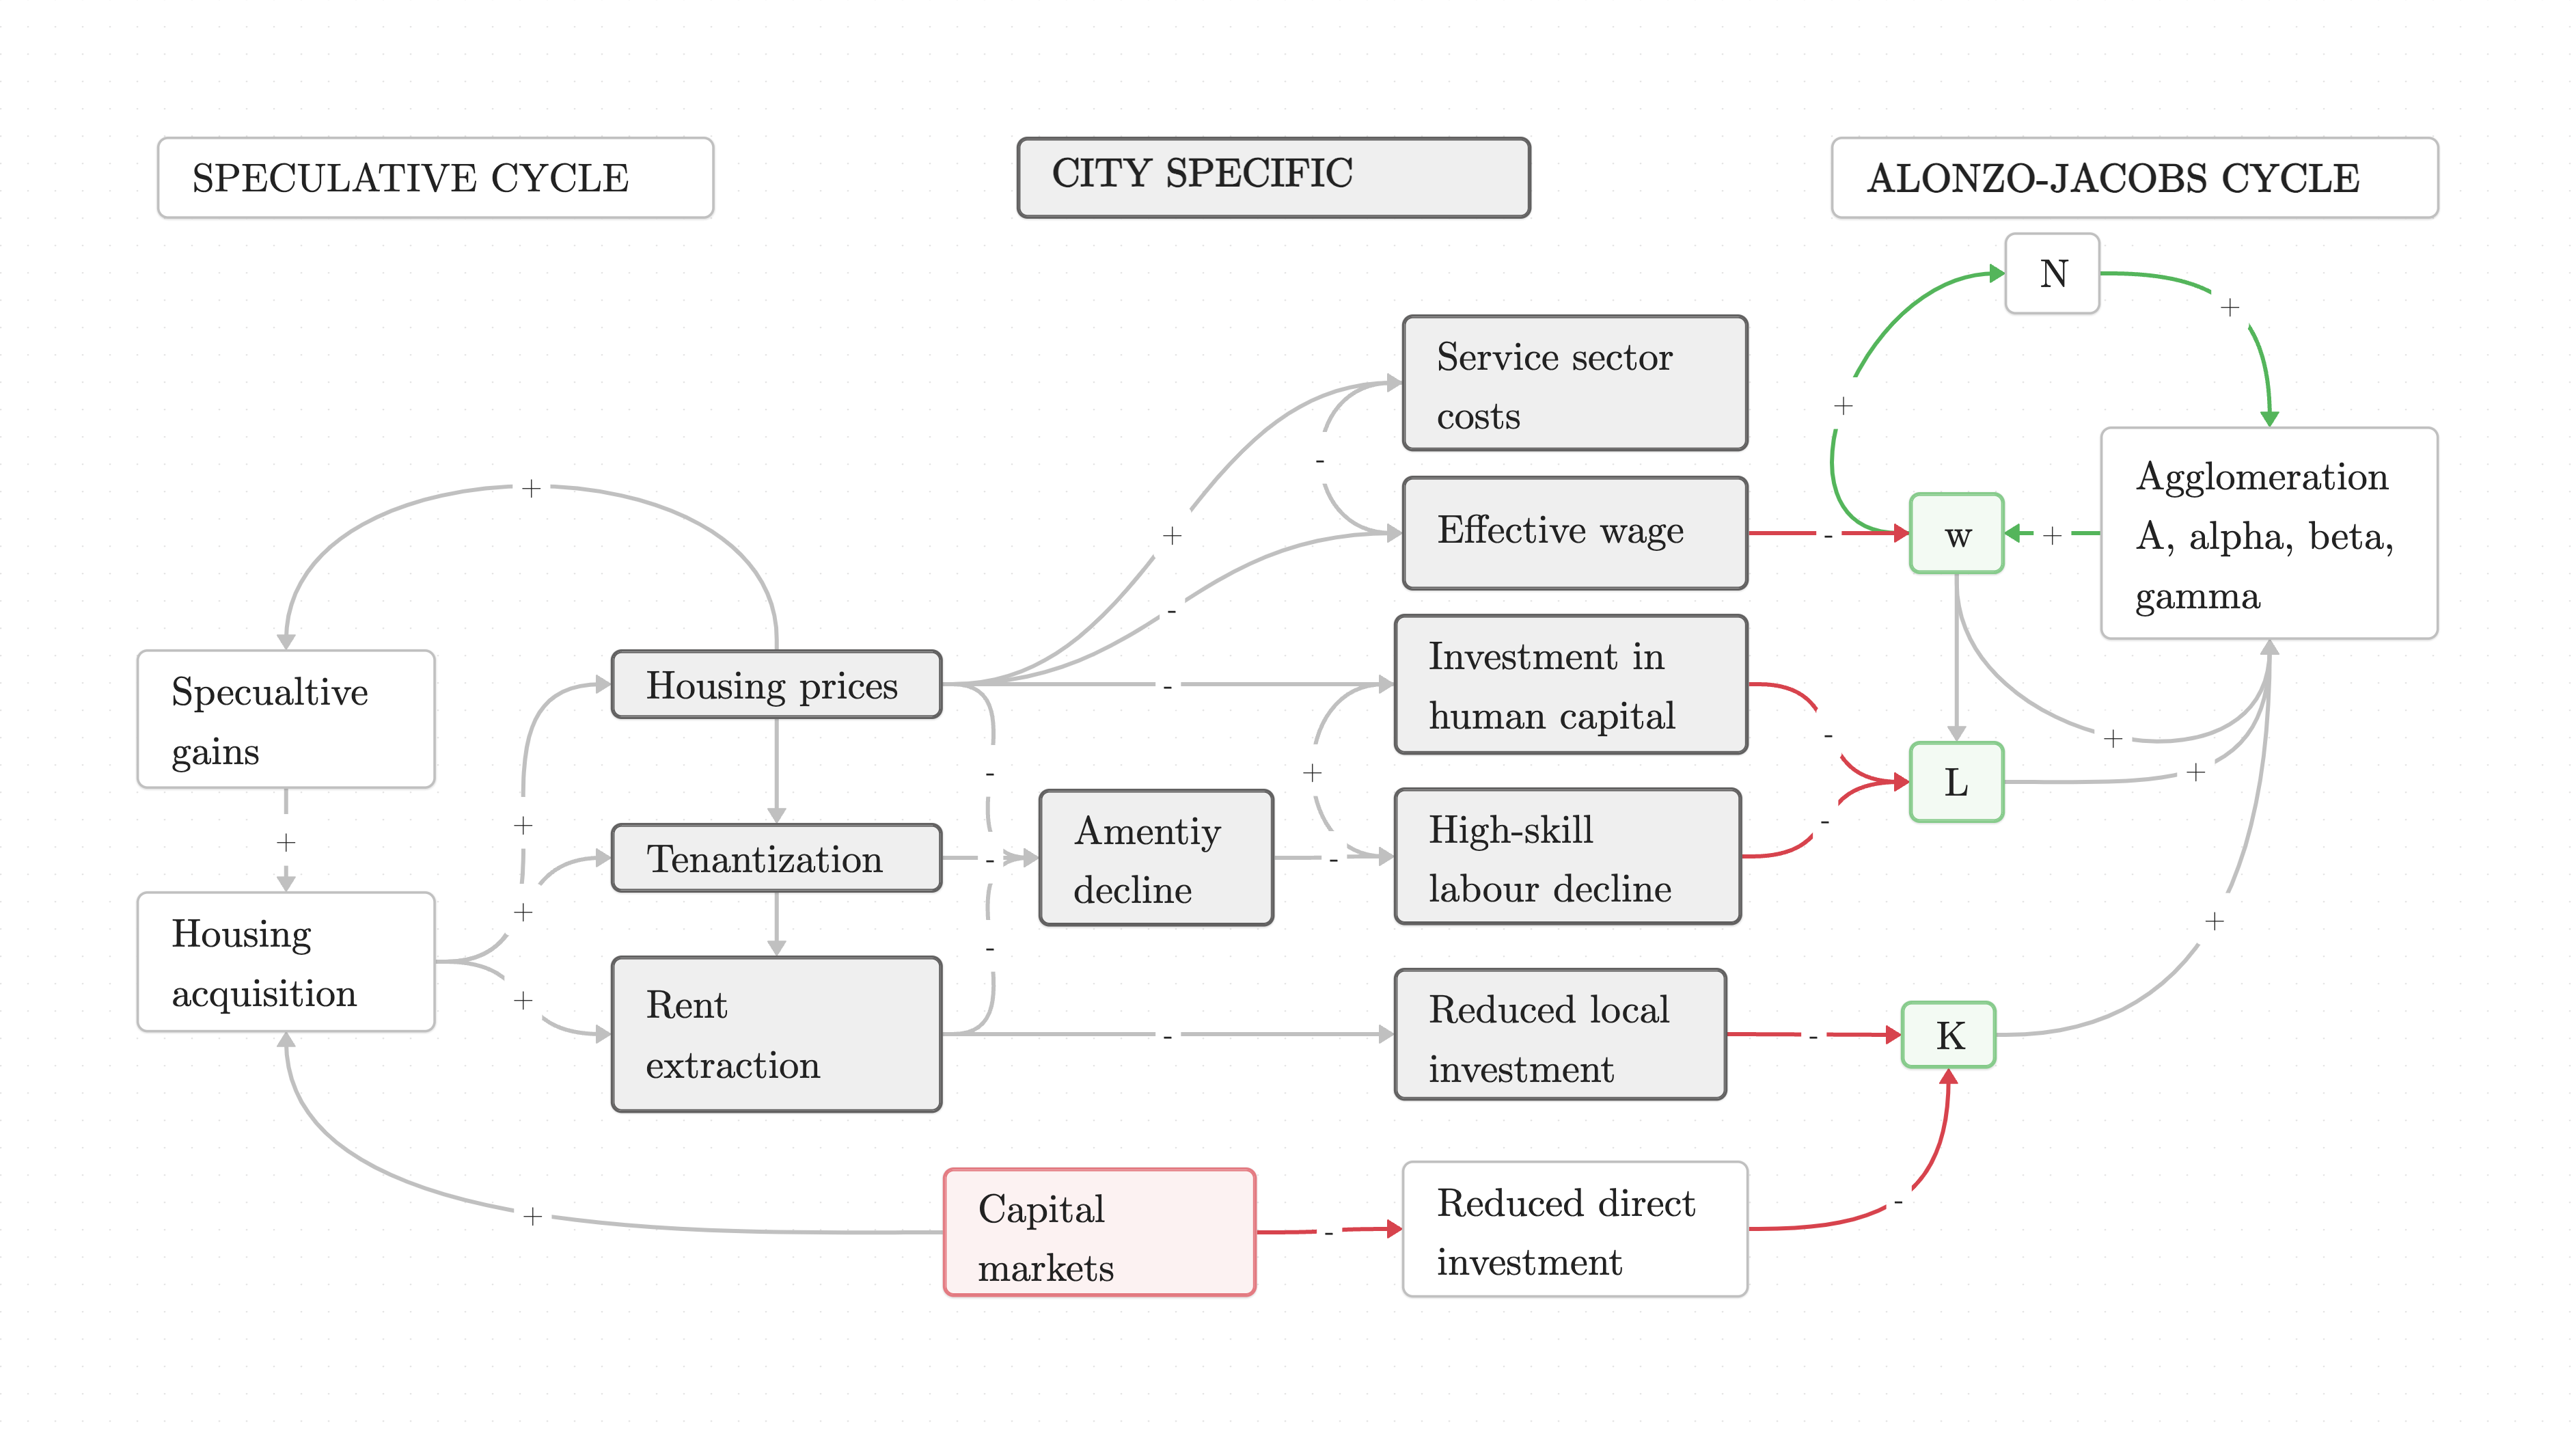
\includegraphics[scale=.15 ]{fig/impact-channels.png}%angle=90
\end{adjustwidth}
\caption[Impact channels relating financialization and urban productivity]{Impact channels relating financialization and urban productivity. Urban production works through the Alonso-Jacobs cycle on the right. For any change in the system to affect output it must at leat one of the variables that regulate the cycle - the capital stock, $K$, effective supply $L$, workers net wage $w$ or  the population  $N$ providing agglomeration effects.}%{\color{red} add K L, w N, alpha beta, gamma - should be symbols- or remove variables?}}
\end{figure}
%}


\section{Policy interventions with a productivity link}

We have suggested that the financialization of the urban housing market may affect urban productivity, laying out plausible links in Chapter~\ref{chapter-tramsmission}. % We explore the potential policy implications of such a link. 
By adding this link to our model, we can explore how it would affect the results of policy interventions. If the model shows that a linkage would have a significant effect on the effectiveness of policy tools, determining whether a link exists, how strong it is, %, if there is a linkage, 
and which channels it operates through become promising targets for urban policy research. 
%Figure~\ref{fig-impact-channels2}, repeated from Chapter~\ref{chapter-tramsmission}, showed that while there are many influences on productivity, in our model, they work through specific parameters of the production function, $y=AN^\gamma k^\alpha n^\beta$. 
The new component in this experiment  %result 
is the formal linkage of the financialized housing market to urban productivity.

To capture the effect of the hypothesized link, we % build in the link between ownership ratio and production by allowing 
make a rising investor share of the housing stock reduce the scale term $A$ in the production function. $A$ is the multiplicative constant term in the Cobb-Douglas production function In the following section, we replace $A$ with:   
\[A^*= (1-0.33s)A,\]
where $s$ is the investor share. $A^*= A$ if the investor share is zero and is reduced by 33\% if the investor share goes to 100\%. $A^*$ thus becomes a dynamic parameter that changes as the model develops.\footnote{The magnitude of the relationship is somewhat arbitrary. %Since we have no empirical studies of the magnitude of the linkages, 
We choose 33\% because it gives values within the range of values for $A$ empirically estimated for cities and large enough to make qualitative impacts easy to see. % Because we do not have empirical estimates about the strengths of the channels through which the productivity effect would work, only the qualitative impacts we illustrate should be taken seriously.  
} 

% \begin{figure}[h!tb]\label{fig-impact-channel-example}
%     \centering
%     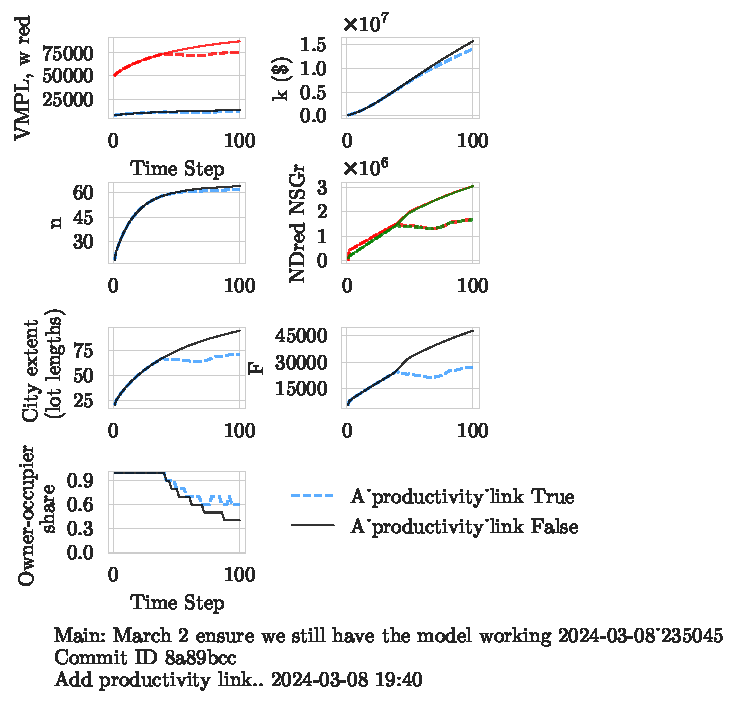
\includegraphics[scale=1, trim=.25cm 2cm .25cm .25cm, clip]{fig/productivity_link.pdf}
%     \caption{Illustrating the impact of financialization on an urban economy}
% \end{figure}


\begin{figure}[h!tb] 
\centering
% \raggedleft
% \hspace{5cm}
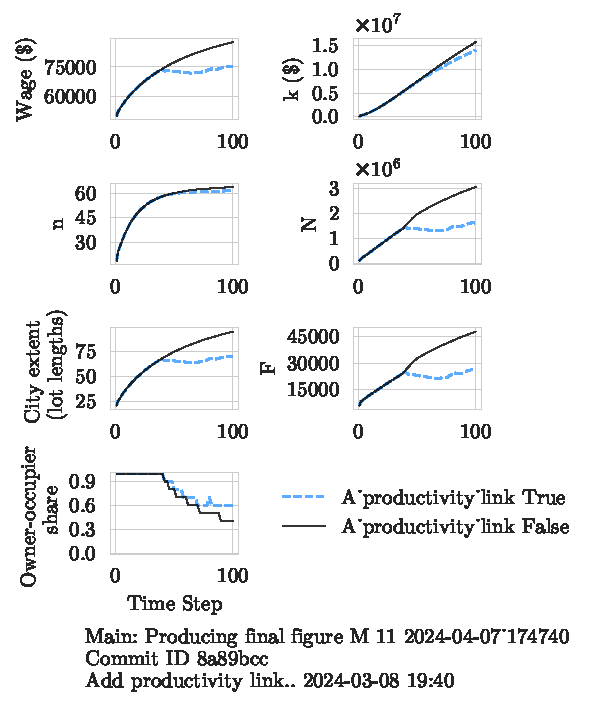
\includegraphics[scale=1, trim={0 1.4cm .0cm 0},clip]{fig/productivity_link_174740.pdf} 
\caption[Productivity linkage in the base model]{The effect of introducing a productivity linkage in the base model. The solid black line shows the case with no linkage, and the dashed blue line shows the case with the productivity linkage. With this linkage, the prefactor value $A$ in the scaling equation is a third, roughly 33\%, lower with 100\% financialized ownership than when property is 100\% owner-occupied. }
\label{fig-impact-channel-example}
\end{figure}

A simulation of this linkage is illustrated in Figure~\ref{fig-impact-channel-example}. The solid black line represents the base case with none of the policy interventions. The dashed blue line shows the effect of introducing the linkage described above. 
The linkage has, as we hypothesized, substantial economic implications. The linkage reduces wages, city size and population.  Declining productivity is the primary channel for this change, which pulls down the wage and the other population variables. The change is amplified by the resulting reduction in aggregation effects. 

There is also a change in ownership share shown in the lower panel of Figure~\ref{fig-impact-channel-example}, where the effect of the linkage reduces the degree of investor ownership. With declining growth, housing investment is less attractive. The model suggests that the linkage is harmful to the economy but the effect on the ownership share is somewhat self-limiting.  If the linkages we have hypothesized exist, the result of financialization would be that we end up with smaller cities with a higher share of owner-occupiers than we would see without the linkage. %\footnote{We cannot conclude that workers are worse off ---  a migration equilibrium ensures all residents are indifferent between urban and rural life. City growth yields capital gains for the original owners but not for newcomers once the population stabilizes.}
%This is, to our knowledge, a new result, although it is consistent with fundamental urban theory and with the trends we see today in the urban system. 

% A simulation of this linkage is illustrated in Figure~\ref{fig-impact-channel-example}.
In the sections below, we analyze the effect of the productivity linkage on the function of policy interventions, by repeating the experiments above with the linkage in place.  %, by policy implications of introducing the productivity linkage in our model, we in the sections below. 
We examine the effect of each policy 
% we will repeat the seven policy interventions examined above with  $A^*$. 
% As before, we use separate figures to represent the impact of each policy 
on the trajectory of each of the seven economic variables over time. The results indicate that the effect of public sector policies may differ in the presence of a productivity link, and that further investigation should be on the agenda of researchers. % urban theorists and policy-makers. 


\newpage

\subsection{Capital gains tax on investors with linkage} \label{subsec:CGinvest}

% {\color{red} Why does the ownership decline LESS in the .5 case with the linkage, and what looks like MORE/FASTER in the .0 case? }

Figure ~\ref{fig:CG-invest_link_W-WO-Cost-of-capital} shows that, with or without the productivity link, a capital gains tax on housing speculation will have a powerful effect on the distribution of ownership. While it has little effect on other variables without the linkage, when we introduce a capital gains tax on investors in the presence of the productivity linkage %the intervention affects not just the ownership ratio but the
we see more significant effects on other variables.

\begin{figure}[h!tb]   %.       MODEL TIKZPICTURE
    \centering
    \begin{tikzpicture}
\node[inner sep=0pt] (plain) at (0,0){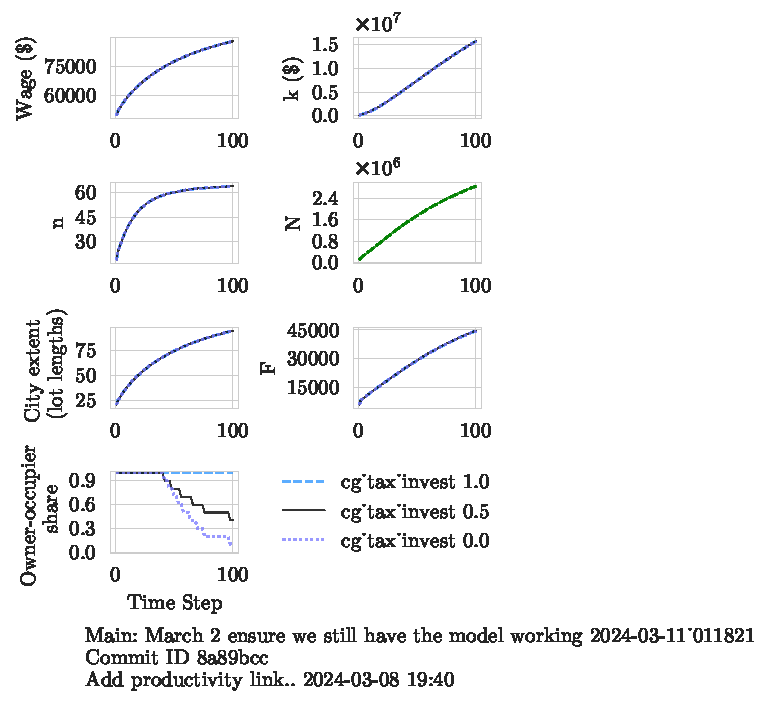
\includegraphics[width=.52\textwidth, trim={.3cm 1.4cm 4.5cm 0},clip]{fig/cg_tax_invest-Main-011821.pdf}}; 

\node[inner sep=0pt] (link) at (8.1,0)
    {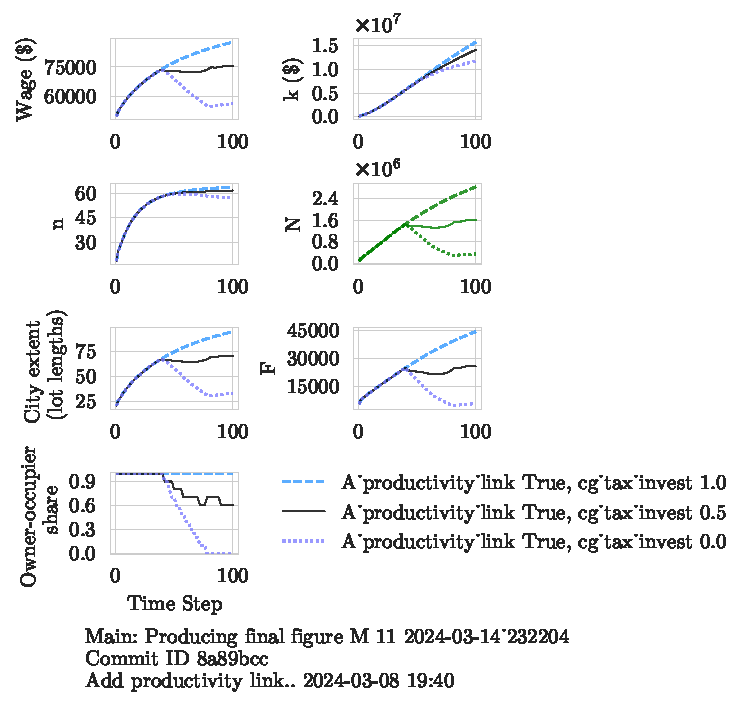
\includegraphics[width=.52\textwidth, trim={0cm 1.4cm 4.3cm 0},clip]{fig/With-productivity_linkcg_tax_invest-232204.pdf}};
    
\draw[color=white, fill=white] (8.5,-2.5) rectangle (12.6,-4.5);
\end{tikzpicture}
    \caption[Capital gains tax for investors with and without linkage]{Comparing the effect of changing the capital gains tax for investors with and without the productivity linkage. This figure illustrates the effect on seven policy variables over time, with a capital gains tax rate for investors of 0\%, 50\%, and 100\%, and the default 1\% rate for homeowners.}
    \label{fig:CG-invest_link_W-WO-Cost-of-capital}
\end{figure}




 % With no productivity link, the capital gains tax rate on land speculation did not affect main economic variables but did affect the ownership ratio. % The dashed line show the effect of a 100\%  tax rate when a link to productivity is present. 
%{\color{red} MAYBE SAY WHAT YOU DO HERE BEFORE ADDING COMPARISON TO THE VERSION WITH NO LINKAGE? ALSO SAY WHAT THE LINE REPRESENT TO START?? 
%A 100\% capital gains tax on speculation with the linkage produces the same outcome for the production economy as any value of the capital gains tax with no linkage. The dotted line illustrates the effect of no capital gains tax on land speculation. In essence, 
% The elimination of the capital gains tax on speculation crashes the economy. % The effect kicks in when 
With the productivity linkage, when the ownership ratio drops dramatically, %as shown by the dotted line in ~\ref{fig:CG-invest_link_W-WO-Cost-of-capital},
% Without a linkage, other variables are unaffected. With a productivity linkage, the feedback from the distribution ownership to the production economy has a powerful effect on the city's production. The linkage means 
the falling owner-occupier rate reduces productivity to a level where increasing returns to the population are offset by decreasing productivity, effectively crashing the local economy. % Keep in mind that we have simply demonstrated the logical possibility of a crash, not that any city is near this point. 
% Both with and without the linkage, a 100\% capital gains tax on land speculation entirely eliminates investor participation. % in the market, leaving 100\%  owner-occupiers. 
On the other hand, a 100\% capital gains tax on land speculation is one of the few interventions that can entirely eliminate investor participation in the housing market, and thus leave  100\%  owner-occupancy, the dashed line in the lower left of the same figure. %,  Figure~\ref{fig:CG-invest_link_W-WO-Cost-of-capital}. %Figure~\ref{fig:Productivity_link_and_CG}
 %Without any tax, owner-occupiers are entirely eliminated, and there is no negative impact on production or city size.  
With a 100\% capital gains tax on speculation, wages are higher, the city is larger, and there are more firms. 
This experiment demonstrates that policy parameters are likely to have different effects when there is a link between financialization and urban productivity and when there is no link.


% \subsubsection{Capital gains tax on investors}

% \begin{figure}[h!tb]
%     \centering
%      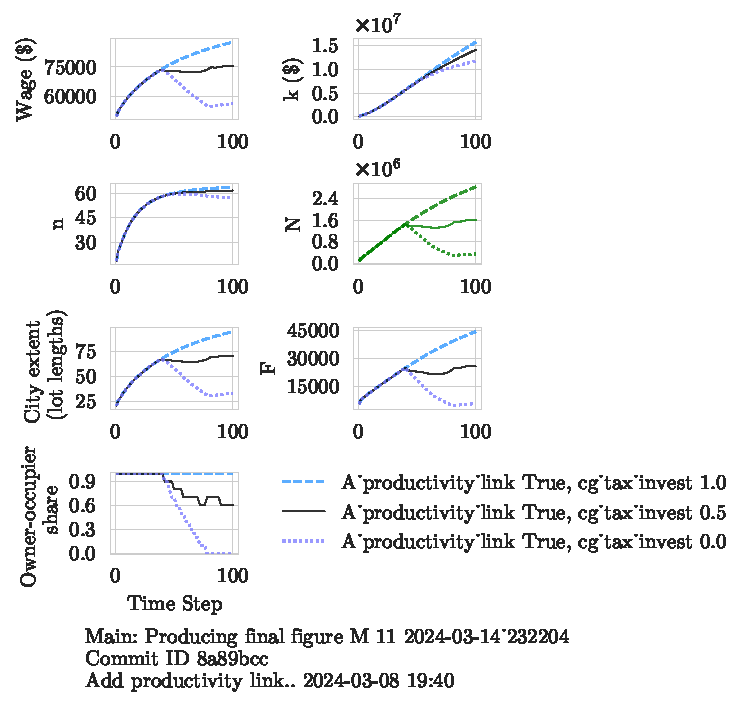
\includegraphics[scale=1, trim=.25cm 2cm .25cm .25cm, clip]{fig/With-productivity_linkcg_tax_invest-232204.pdf}
%     \caption[Capital gains tax for investors with linkage]{The effect of changing the capital gains tax for investors with a productivity linkage. Illustrates the effect on seven policy variables over time, with a capital gains tax rate of 0\%, 50\%, and 100\% for investors, and the default 1\% rate for homeowners.}
%     \label{fig:Productivity_link_and_CG}
% \end{figure}


% \begin{figure}[h!tb] 
%     \centering
%     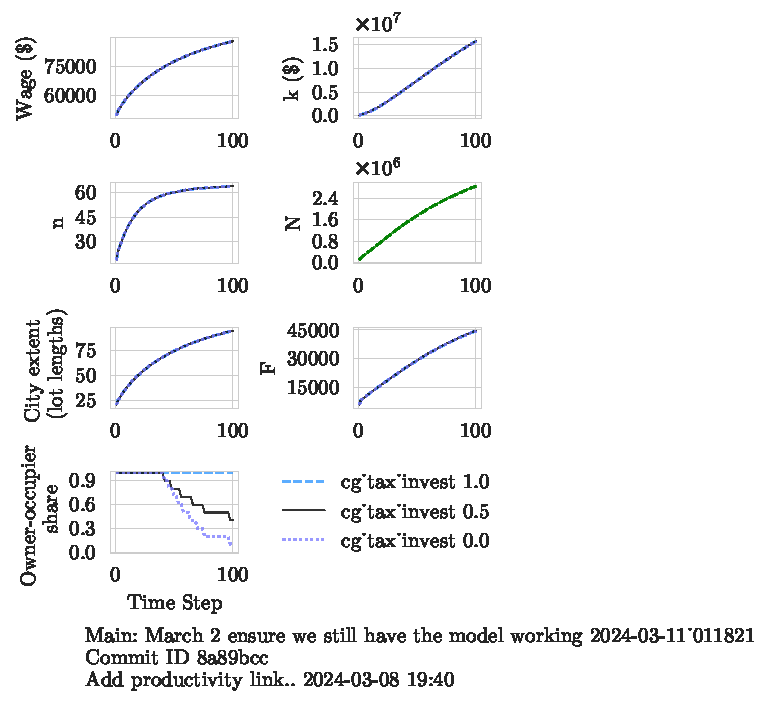
\includegraphics[scale=.75, trim={0 1.4cm 4.5cm 0},clip]{fig/cg_tax_invest-Main-011821.pdf} 
%     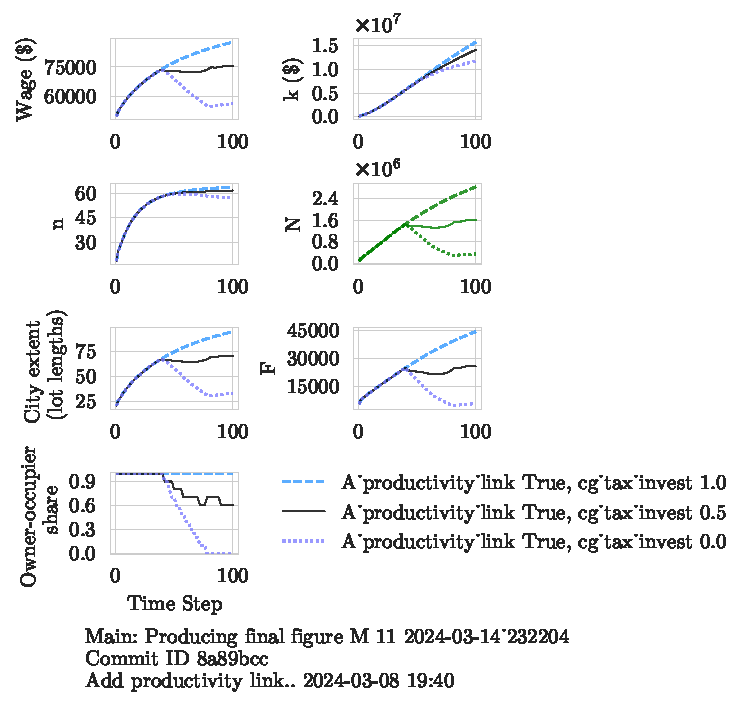
\includegraphics[scale=.75, trim={0 1.4cm 3.7cm 0},clip]{fig/With-productivity_linkcg_tax_invest-232204.pdf} 
   
% \end{figure}


\newpage
\subsection{Capital gains tax on owner-occupiers  with linkage}
% {\color{red} MAKE SURE EXPLANATION IS CONSISTENT WITH ABOVE..}
In this subsection, we explore the effect of a capital gains tax for owner-occupiers in the presence of linkages. 
% In Figure~\ref{fig:CG-pers_link_W-WO-Cost-of-capital}, %{fig:Productivity_link_and_CGpers_ownership_trajectory}, 
% the capital gains tax on investors is set at 15\% and we vary the capital gains tax on owner-occupiers. 
In Figure~\ref{fig:CG-pers_link_W-WO-Cost-of-capital}, the dotted line represents the case with no capital gains tax for homeowners, the solid line represents a 50\% tax, and the dashed line represents a 100\% tax.
\begin{figure}[h!tb]   
    \centering
    \begin{tikzpicture}
\node[inner sep=.5pt] (plain) at (0,0)
    {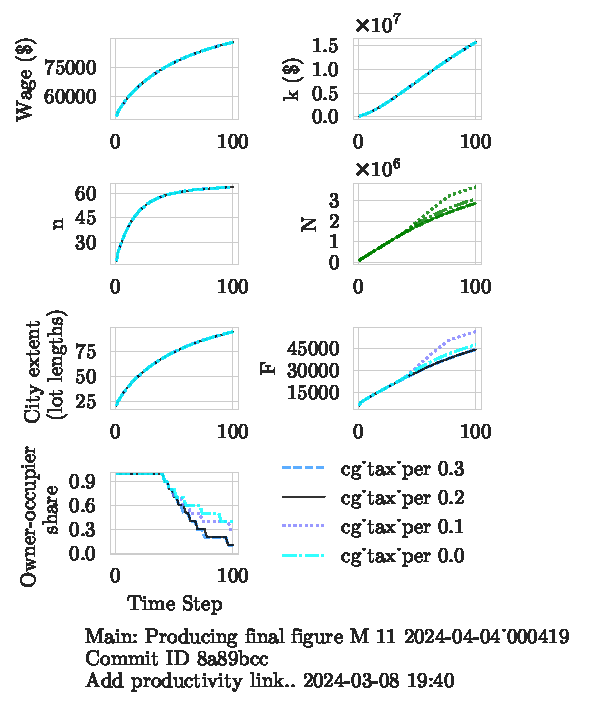
\includegraphics[height=10cm,%width=.5\textwidth,
    trim={.3cm 1.4cm 1cm 0},clip]{fig/cg_tax_per-000419.pdf}}; 

\node[inner sep=0pt] (link) at (8.1,0)
    {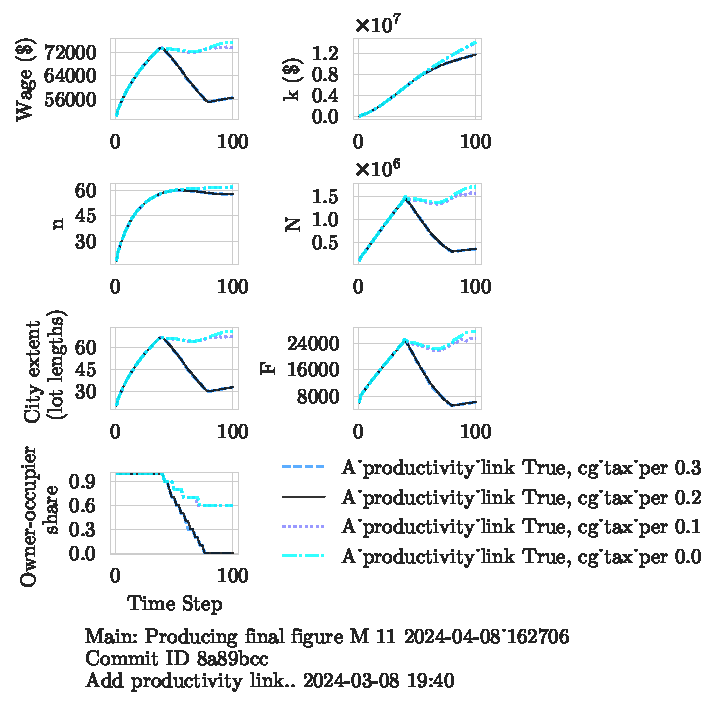
\includegraphics[height=10cm,%width=.5\textwidth, 
    trim={.1cm 1.4cm 4.cm 0},clip]{fig/link-cg_tax_per-4_162706.pdf}};
    
\draw[color=white, fill=white] (8.3,-2.3) rectangle (12.6,-4.5);
\end{tikzpicture}
     \caption[Capital gains tax for owner-occupiers with and without a linkage]{Comparing the effect of introducing a capital gains tax for owner-occupiers with and without a productivity linkage. this figure illustrates the effect on seven policy variables over time, with a capital gains tax rate of 0\%, 10\%, 20\% and 30\% for owner-occupiers, and the default 15\% rate for investors.}
    \label{fig:CG-pers_link_W-WO-Cost-of-capital}
\end{figure}
Taxing capital gains tax for owner-occupiers advantages investors. 
% When the tax is higher than the rate for investors, 
A higher capital gains tax on homeowners than investors %shown by the solid and the dashed lines, 
results in home ownership falling substantially more than when it is lower. It also results in a much lower population and city size, which leads to lower rents for tenants because locational rents are lower. The sensitivity of the model economy to capital gains taxes on owners suggests a need for further research. 

There is some rebound from the lowest level. 
With a productivity link, a high relative tax rate produces a city that rises rapidly and then declines. Slow growth begins after the decline. The economic variables decline rapidly, % and overshoot slightly. The 
then city extent, wage and firm count all recover slightly from their initial decline. % {\color{red} EXPLAIN THIS REBOUND.} 
% {\color{red}
% LOOK AT DIFFERENT VARIABLES WITH THE PRODUCTIVITY LINK..
% MAYBE WE ARE MISSING A SECTION RUNNING THE MODEL WITH THE PRODUTIVITUY LINK - MAYBE ON/OFF - BUT WITHOUT ANY INTERVENTION... WE JUST SHOW WHAT HAPPENS IN THE MODEL WITH JUST TURNING PRODUCTIVITY ON
% SAY 'THE OWNERSHIP RESULT IS THE SAME, BUT THERE ARE EFFECTS ON THESE OTHER THINGS..'
% }
% \subsubsection{Capital gains tax on owner-occupiers}
%{\color{red} THIS FIGURE IS LABELLED COST OF CAPITAL NOT CAP GAINS Figure ~\ref{fig:CG-pers_link_W-WO-Cost-of-capital} } shows that, 
Regardless of the presence or absence of a productivity link, when the capital gains tax on homeowners is above the rate of investors, %shown by the overlapping solid, dashed, and dotted lines,  
home ownership falls farther and faster than when it is lower than the investor rate. 
It drops a bit as a result of the increase in investor-owned population. There is a bit of a wobble after that, and that's because the population grows a little bit after that. The rebound occurs because financialization actually appears to suppress growth for a period, and then growth starts to come back over time. 


% \begin{figure}[h!b]
%     \centering
%     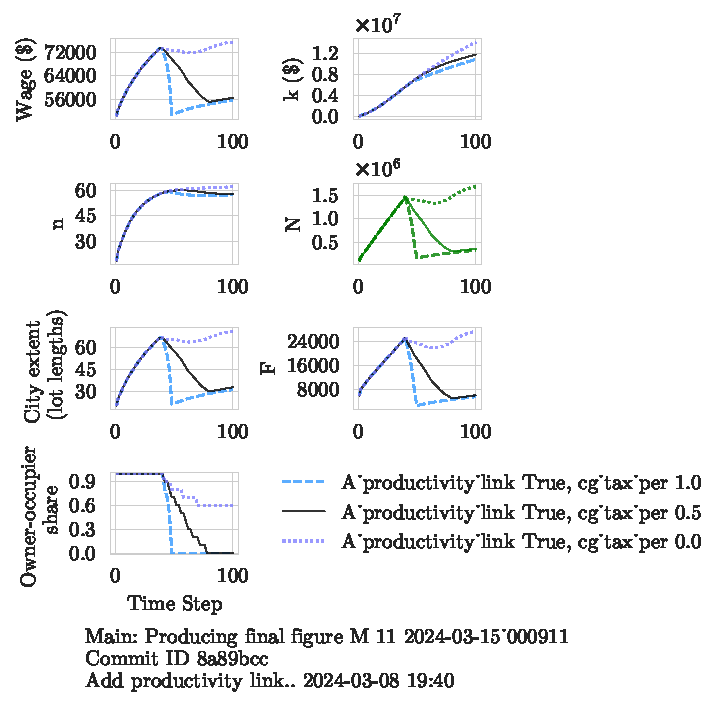
\includegraphics[scale=1, trim={0 1.4cm 0 0},clip]{fig/With-productivity_link_cg_tax_per-000911.pdf}
%     \caption[Capital gains tax for owner-occupiers with a productivity linkage]{The effect of introducing a capital gains tax for owner-occupiers with a productivity linkage. Illustrates the effect on seven policy variables over time, with a capital gains tax rate of 0\%, 10\%, 20\% and 30\% for owner-occupiers, and the default 15\% rate for investors.}
%     \label{fig:Productivity_link_and_CGpers_ownership_trajectory}
% \end{figure}



% \begin{figure}[h!tb] 
%     \centering
%     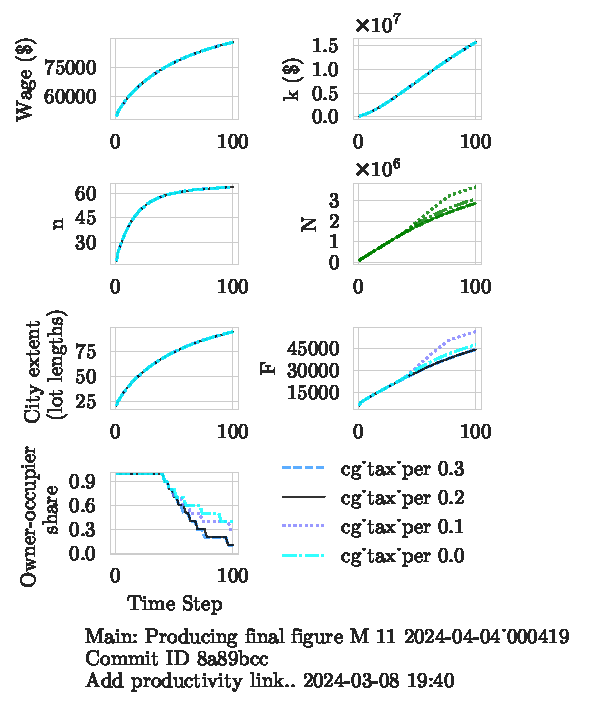
\includegraphics[scale=.75, trim={0 1.4cm .5cm 0},clip]{fig/cg_tax_per-000419.pdf} 
%     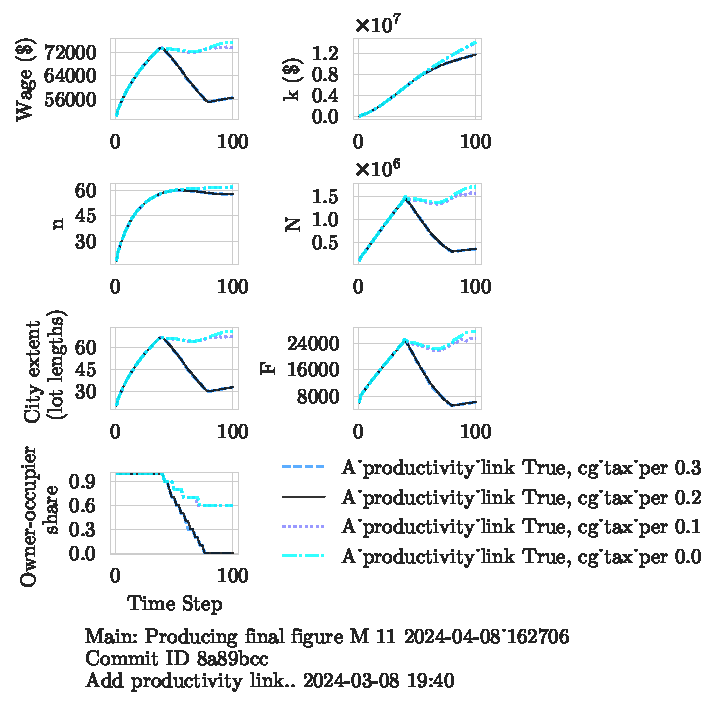
\includegraphics[scale=.75, trim={0 1.4cm 3.5cm 0},clip]{fig/link-cg_tax_per-4_162706.pdf}% With-productivity_link_cg_tax_per-000911.pdf
%     \caption[Capital gains tax for owner-occupiers with and without a productivity linkage]{The effect of introducing a capital gains tax for owner-occupiers with and without a productivity linkage. Illustrates the effect on seven policy variables over time, with a capital gains tax rate of 0\%, 10\%, 20\% and 30\% for owner-occupiers, and the default 15\% rate for investors, comparing a productivity linkage and no productivity linkage.}
%     \label{fig:CG-pers_link_W-WO-Cost-of-capital}
% \end{figure}







\newpage
\subsection{The cost of capital for investors  with linkage}
% 'r_investor': [0.2, 0.1, .05] has set up for morning
Figure ~\ref{fig:Productivity_link_W-WO-Cost-of-capital} %{fig:Productivity_link_and_capital_ownership_trajectory} 
shows the effect of increasing capital costs for investors. Even in the presence of strong productivity spillovers, it has little effect in this experiment which suggests that the cost of capital for investors is dominated by other factors in this model. The low effect on ownership means even with the linkage in place, it has less effect on other economic variables. 
% \subsubsection{The cost of capital for investors}
\begin{figure}[h!tb]   
    \centering
    \begin{tikzpicture}
\node[inner sep=.5pt] (plain) at (0,0)
    {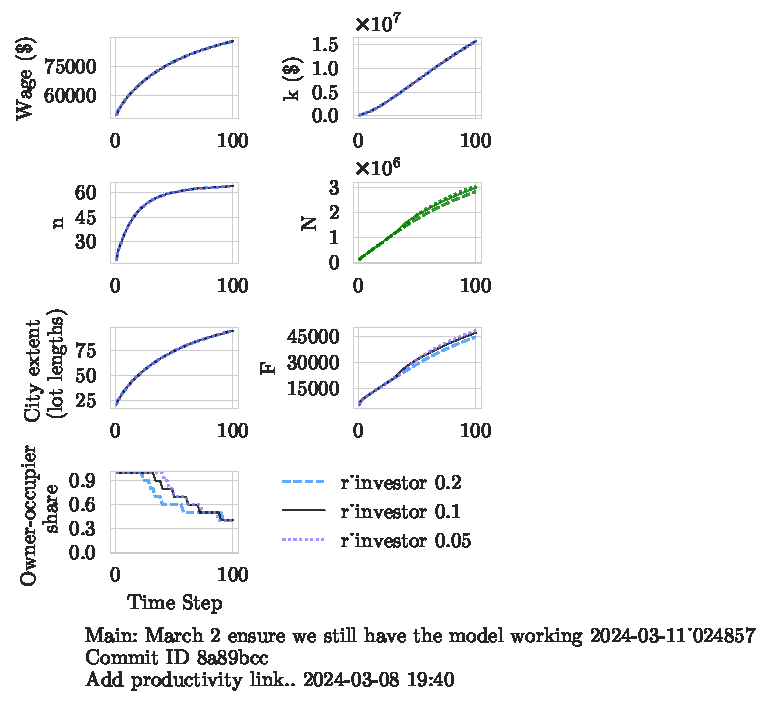
\includegraphics[height=10cm,%width=.5\textwidth,
    trim={.3cm 1.4cm 1cm 0},clip]{fig/r_investor-Main-024857.pdf}}; 

\node[inner sep=0pt] (link) at (6.4,0)
    {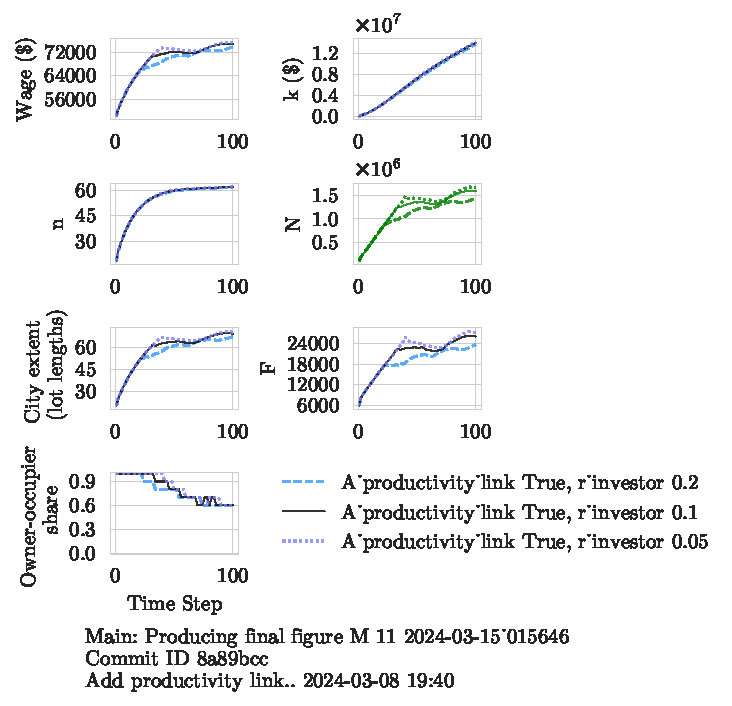
\includegraphics[height=10cm,%width=.5\textwidth, 
    trim={.1cm 1.4cm 4.cm 0},clip]{fig/With-productivity_link-r_investor-15_015646.pdf}};
    
\draw[color=white, fill=white] (7,-2.3) rectangle (10.6,-4.5);
\end{tikzpicture}
     \caption[Capital costs for investors with and without linkage]{Comparing the effect of raising capital costs for investors with and without a productivity linkage. Illustrates the effect on seven policy variables over time, with an investor rate of 5\%, 10\% and 20\%, and a rate for owner-occupiers near 5.1\%, just above the bank's prime rate, adjusted based on individual assets and income.}
    \label{fig:Productivity_link_W-WO-Cost-of-capital}
\end{figure}
% {\color{red}Without the productivity linkage??, YOU SAY BELOW THAT IT IS 20 percent Different?} 
Higher capital costs for investors appear to increase the speed at which the effects take place but do not affect the final level of investor ownership. Productivity spillovers cut population and wages, keep the owner-occupier share just 20\% higher, and introduce what may be a weak speculative cycle. %The cost of capital for investors does not appear to be a promising policy tool.
% \begin{figure}[h!t]
%     \centering
%    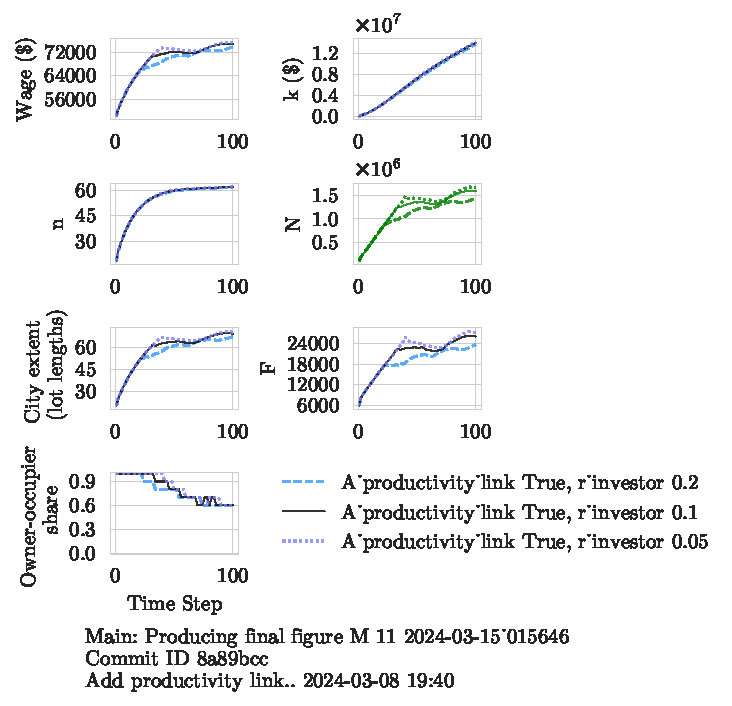
\includegraphics[scale=1, trim={0 1.4cm 0 0},clip]{fig/With-productivity_link-r_investor-15_015646.pdf}
%     \caption[Raising capital costs for investors with a productivity linkage]{The effect of raising capital costs for investors with a productivity linkage. Illustrates the effect on seven policy variables over time, with an investor rate of 5\%, 10\% and 20\%, and a rate for owner-occupiers near 5.1\%, just above the bank's prime rate, adjusted based on individual assets and income.}
%     \label{fig:Productivity_link_and_capital_ownership_trajectory}
% \end{figure}

% \begin{figure}[h!tb] 
%     \centering
%     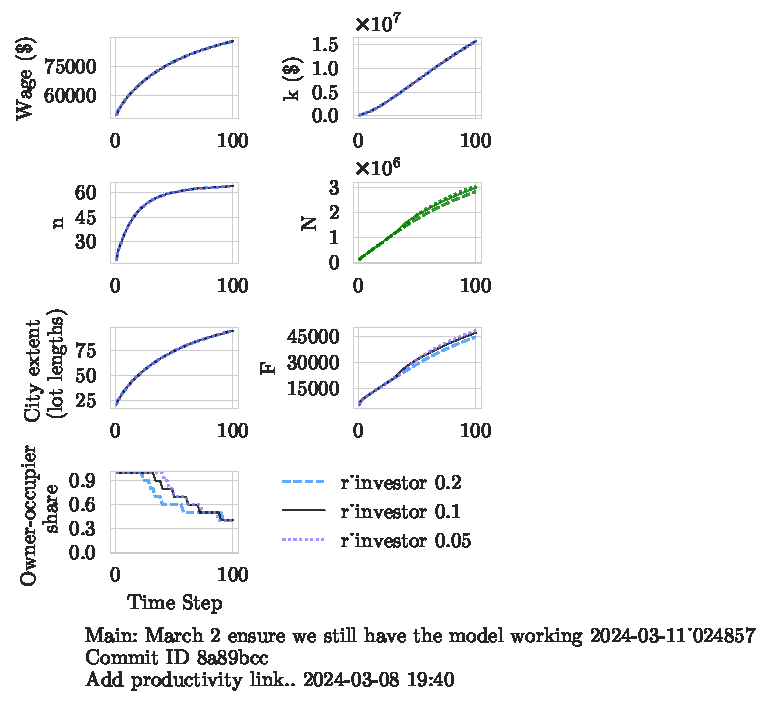
\includegraphics[scale=.75, trim={0 1.4cm 4cm 0},clip]{fig/r_investor-Main-024857.pdf} 
%     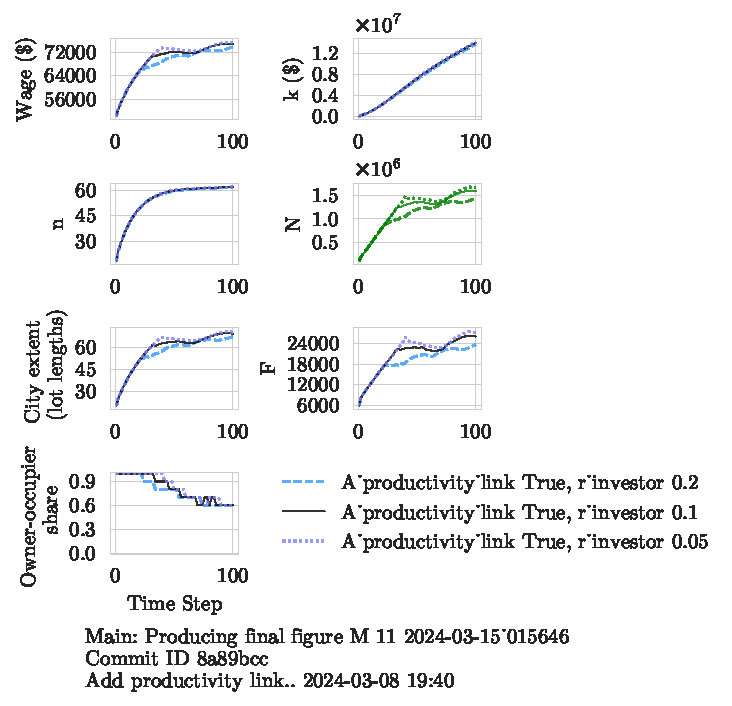
\includegraphics[scale=.75, trim={0 1.4cm 3.5cm 0},clip]{fig/With-productivity_link-r_investor-15_015646.pdf} 
%     \caption[Raising capital costs for investors with and without a productivity linkage]{The effect of raising capital costs for investors with and without a productivity linkage. Illustrates the effect on seven policy variables over time, with an investor rate of 5\%, 10\% and 20\%, and a rate for owner-occupiers near 5.1\%, just above the bank's prime rate, adjusted based on individual assets and income.}
%     \label{fig:Productivity_link_W-WO-Cost-of-capital}
% \end{figure}

\newpage

\subsection{Transportation costs  with linkage}\label{subsec-transport-link}

In Figure~\ref{fig:Productivity_link_W-WO-transportation-cost}, we reduce transportation costs for everyone by 40\%, this time in the presence of productivity impact. The linkage reduces wages and city size to the base case without the linkage, but city size and population increase with lower transportation costs as expected. The linkage also introduces large oscillations in population and city size.  %The oscillations are discussed in section~\ref{subsec-transport-pair}, where we put the two sets of results side by side. 



% \begin{figure}[h!t]
%     \centering
%     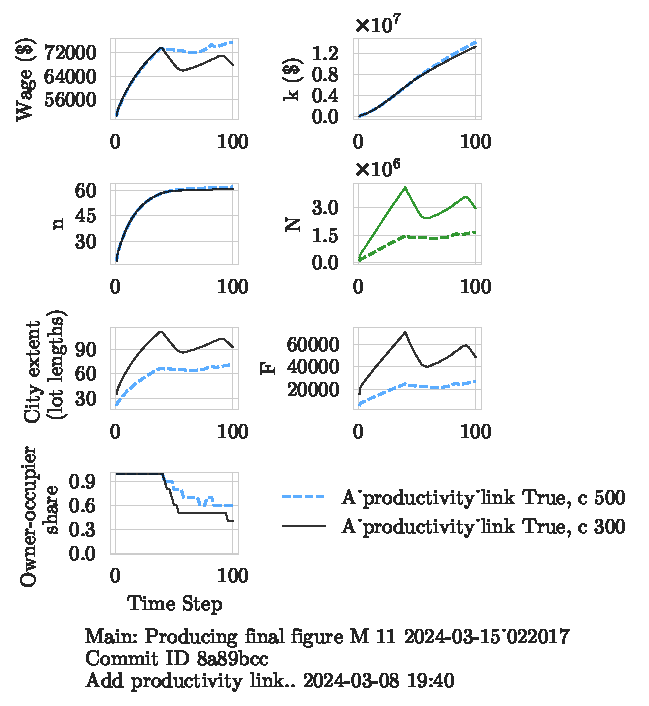
\includegraphics[scale=1, trim={0 1.4cm 0 0},clip]{fig/With-productivity_link-c-15_022017.pdf}
%     \caption[Decreasing transportation costs with linkage]{The effect of decreasing transportation costs with a productivity linkage. Illustrates the effect on seven policy variables over time, with a cost of \$300 and \$500 per unit distance per year.}
%     \label{fig:Productivity_link_and_c_ownership_trajectory}
% \end{figure}
\begin{figure}[h!tb]   
\centering
\begin{tikzpicture}
\node[inner sep=.5pt] (plain) at (-2,0)
{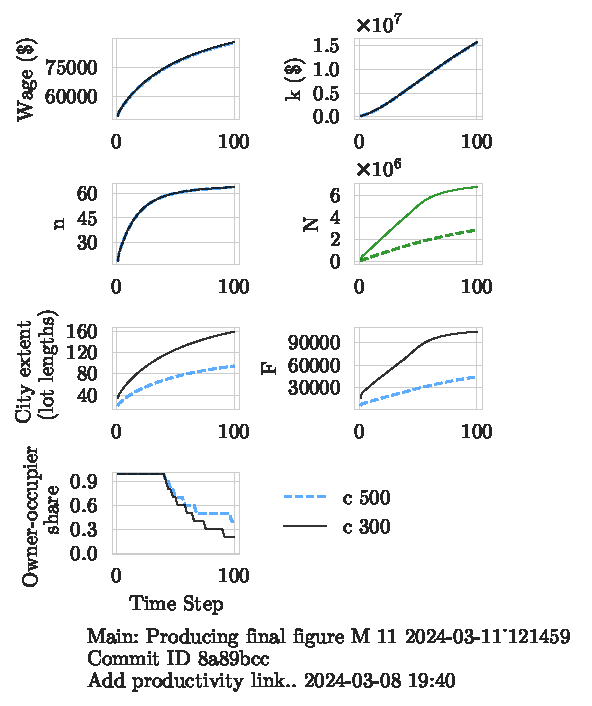
\includegraphics[height=10cm,%width=.5\textwidth,
trim={.2cm 1.4cm 1cm 0},clip]{fig/c-Main-121459.pdf}}; 

\node[inner sep=0pt] (link) at (6,0)
{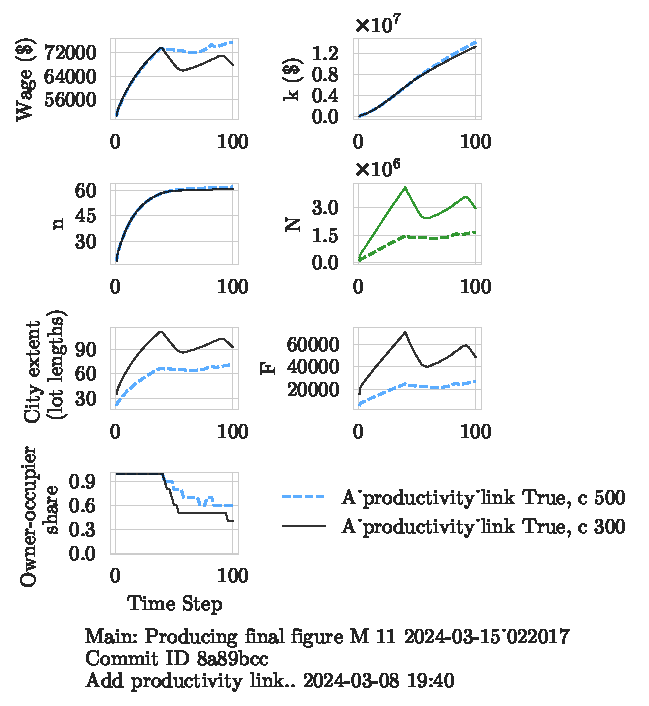
\includegraphics[height=10cm,%width=.5\textwidth, 
trim={0cm 1.4cm 2.5cm 0},clip]{fig/With-productivity_link-c-15_022017.pdf}};

\draw[color=white, fill=white] (6,-2.3) rectangle (10.2,-4.5);
\end{tikzpicture}
\caption[Decreasing transportation costs with and without linkage]{Comparing the effect of decreasing transportation costs with and without a productivity linkage. This figure illustrates the effect on seven policy variables over time,  under circumstances where transportation costs \$300 and \$500 per unit distance per year.}
\label{fig:Productivity_link_W-WO-transportation-cost}
\end{figure}
With or without productivity links, lower transportation costs decrease the home-ownership ratio. 
% Lower transportation costs produces a lower home-ownership ratio. 
Lower transportation costs lead to higher land rents, which increases property prices and  capital gains, which makes investment more appealing to speculators and ultimately leads to a smaller fraction of owner-occupiers.

A decline in the wage also appears to accompany reduced transport costs. This may be understood by noticing that lower transport costs reduce the wage needed to attract workers to the city, so the size of the city is larger at any given wage level. % {\color{red} BUT WHY IS IT LOWER OVERALL?} 

% \subsubsection{Transportation cost}\label{subsec-transport-pair}

A productivity link reduces wage and population growth in all transportation cost experiments,  but Figure~\ref{fig:Productivity_link_W-WO-transportation-cost} %{fig:Productivity_link_W-WO-transportation-cost}
shows that low transportation costs with a link may produce especially large speculative cycles. %, as pointed out in Subsection~\ref{subsec-transport-link} 
If we look more carefully at the patterns, it appears that the trajectories initially follow those without linkage and then diverge when the ownership ratio drops. A period with stable ownership results in another period of growth, which attracts another round of speculation that further reduces productivity and wages. Smaller irregularities in other experiments are probably due to the same effect. 
% \begin{figure}[h!tb] 
%     \centering
%     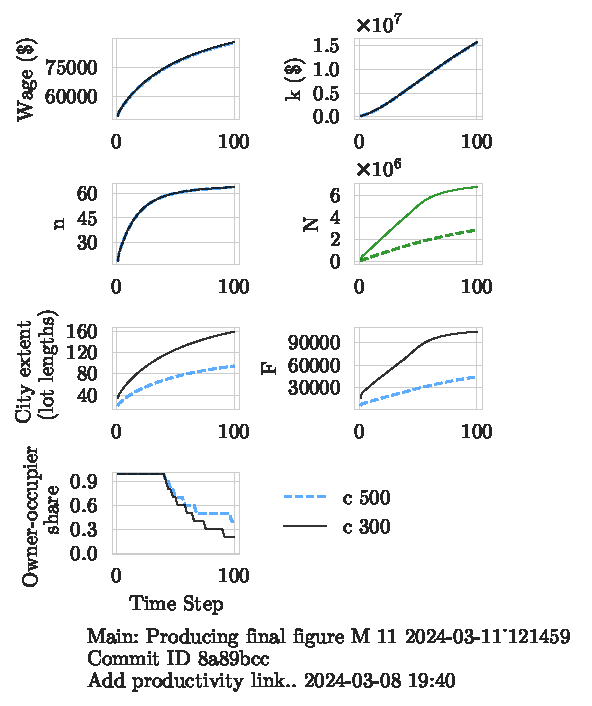
\includegraphics[scale=.75, trim={0 1.4cm 1.5cm 0},clip]{fig/c-Main-121459.pdf} 
%     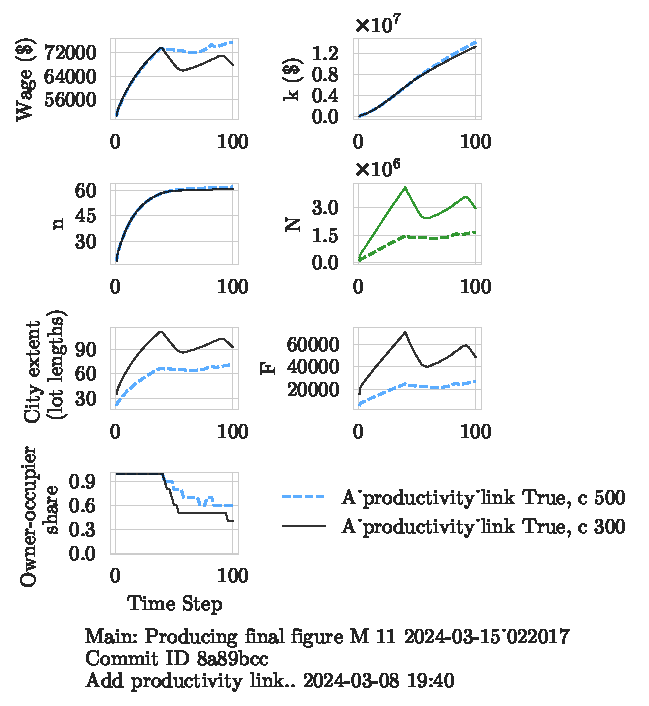
\includegraphics[scale=.75, trim={0 1.4cm 2.3cm 0},clip]{fig/With-productivity_link-c-15_022017.pdf} 
%     \caption[The effect of decreasing transportation costs with and without a productivity linkage]{The effect of decreasing transportation costs with and without a productivity linkage. Illustrates the effect on seven policy variables over time, with a cost of \$300 and \$500  per unit distance per year, comparing a productivity linkage and no productivity linkage.}
%     \label{fig:Productivity_link_W-WO-transportation-cost}
% \end{figure}
% as explained in in Subsection~\ref{subsec-transport-link}. 
%$The decline in the wage that appears to accompany reduced transport costs may be understood by noticing that lower transport costs reduce the wage needed to attract workers to the city. 


\newpage
\subsection{Density with linkage}
% 'density': [100, 150]
Relaxing restrictions on density should, in theory, affect the ability of people to buy homes. Our results indicate that the effect of increasing density is significant but has no effect on city extent and no effect on the ownership ratio. % The first two results are expected, the third less so but easily explained. 
The share of homeowners is not affected, since rent per unit is unchanged at any distance, density alone does not affect the relative advantage of new home buyers and investors, leaving the ratio constant. % There are more homes, however, and, since the relative advantages of owners and investors are unchanged, additional homes are distributed the same way as with lower density.  
% {\color{red} NEED THIS? Density does not affect transportation cost, and in this test version firm size is not affected. The number of firms rises instead. }
With productivity links, wages are depressed, and population is lower and appears to cycle.
\begin{figure}[h!tb]   
    \centering
    \begin{tikzpicture}
\node[inner sep=.5pt] (plain) at (-2,0)
    {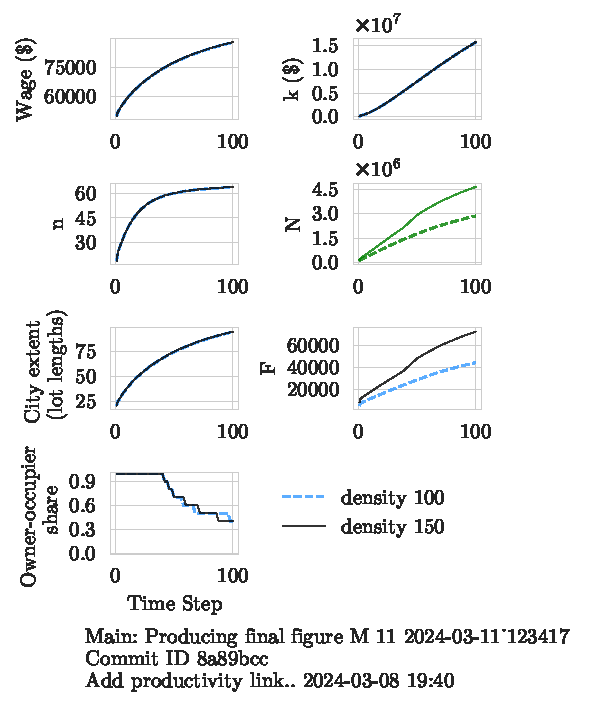
\includegraphics[height=10cm,%width=.5\textwidth,
    trim={.2cm 1.4cm 1cm 0},clip]{fig/density-Main-123417.pdf}}; 

\node[inner sep=0pt] (link) at (6,0)
    {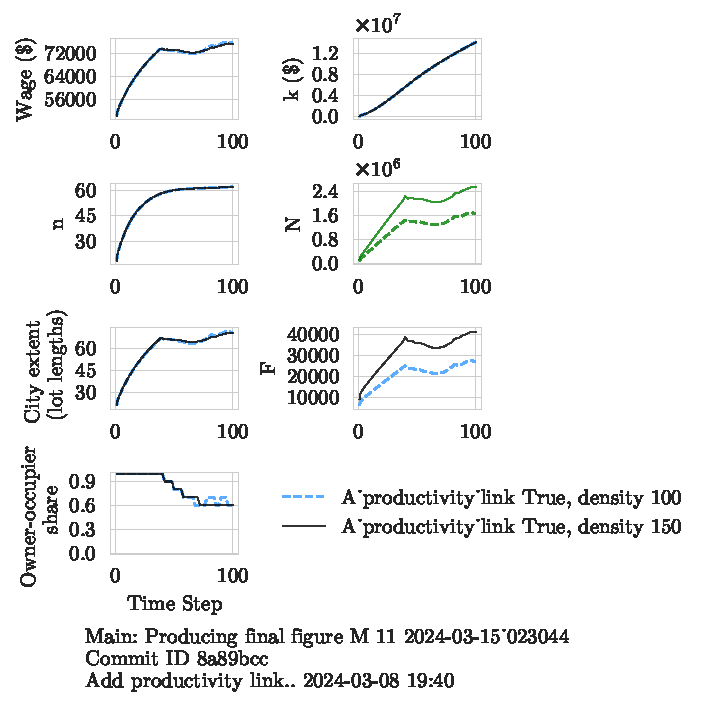
\includegraphics[height=10cm,%width=.5\textwidth, 
    trim={0cm 1.4cm 3.5cm 0},clip]{fig/With-productivity_link-density-023044.pdf}};
    
\draw[color=white, fill=white] (6,-2.3) rectangle (10.2,-4.5);
\end{tikzpicture}
      \caption[Increasing density with and without linkage]{Comparing the effect of increasing density with and without a productivity linkage. Illustrates the effect on seven policy variables over time, with a population density of 100 and 150 per grid space.}
    \label{fig:Productivity_link_W-WO-density}
\end{figure}
% \subsubsection{Density}
% The effect of density on city population is significant but it has no effect on city extent and no effect on the ownership ratio. The share of homeowners is not affected although the number of homes is. 
% \begin{figure}[h!tb] 
%     \centering
%     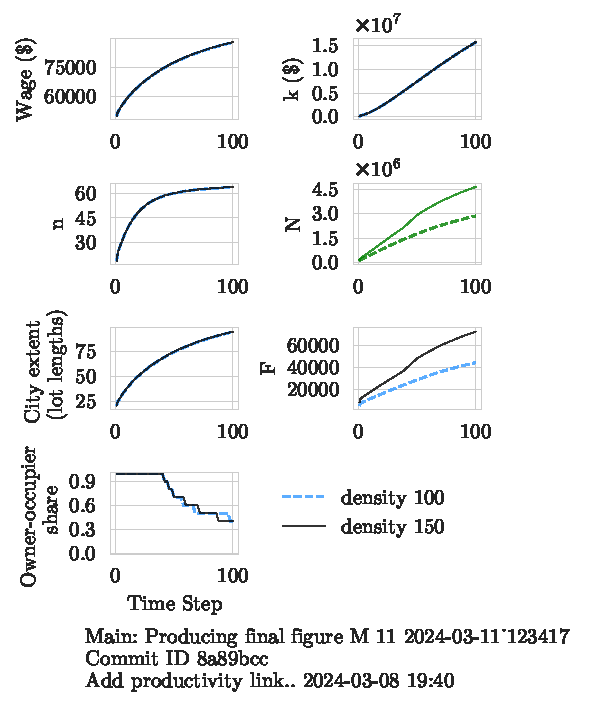
\includegraphics[scale=.75, trim={0 1.cm 1.5cm 0},clip]{fig/density-Main-123417.pdf} 
%     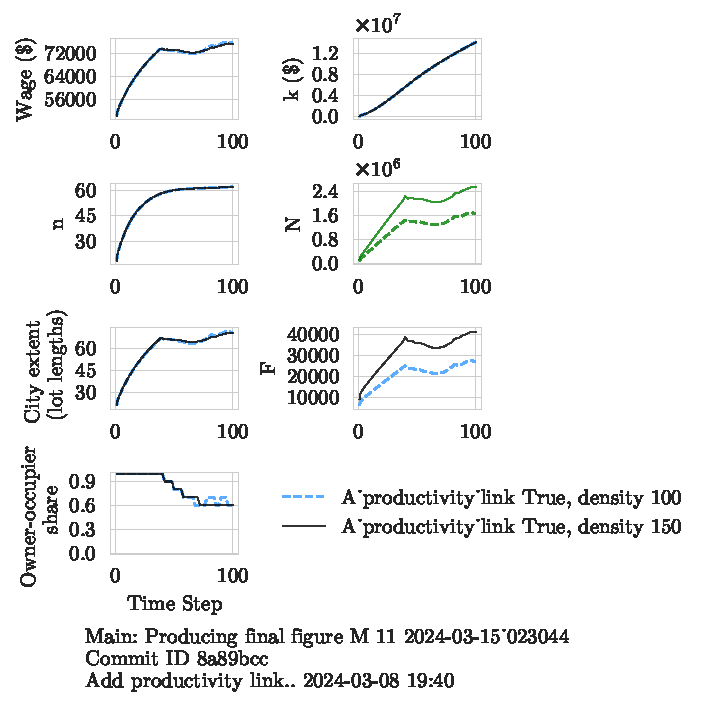
\includegraphics[scale=.75, trim={0 1.4cm .2cm 0},clip]{fig/With-productivity_link-density-023044.pdf} 
%     \caption[The effect of increasing density with and without a productivity linkage]{The effect of increasing density with and without a productivity linkage. Illustrates the effect on seven policy variables over time, with a population density of 100 and 150 per grid space, comparing a productivity linkage and no productivity linkage.}
%     \label{fig:Productivity_link_W-WO-density}
% \end{figure}
\newpage

\subsection{Cost of financing's dependence on borrower's wealth with linkage}

In Figure~\ref{fig:Productivity_link_W-WO-wealth} %{fig:Productivity_link_and_wealth_sensitivity_ownership_trajectory} 
we vary the wealth sensitivity in the presence of a productivity linkage. The higher value is more restrictive, lowering the threshold so more assets are required to secure a mortgage. % harder for someone without assets to get a mortgage. 
The intervention has no substantial effect on the ownership ratio. % {\color{red} this is very abrupt? ADD OTHER MARKERS SUMMARY}
% {\color{red} MAYBE ADD A SUMMARY OF THIS SECTION SAYING THAT THE POLICIES/HOW WE UNDERSTAND THEM SHOULD CHANGE DEPENDING ON WHETHER THERE IS THIS PRODUCTIVITY LINK...}
% 'wealth_sensitivity': [0.15, 0.1, 0.5]r
% \subsubsection{Cost of financing's dependence on borrower's wealth}
\begin{figure}[h!tb]   %.      first version of  TIKZPICTURE
\centering
\begin{tikzpicture}
\node[inner sep=0pt] (plain) at (0,0){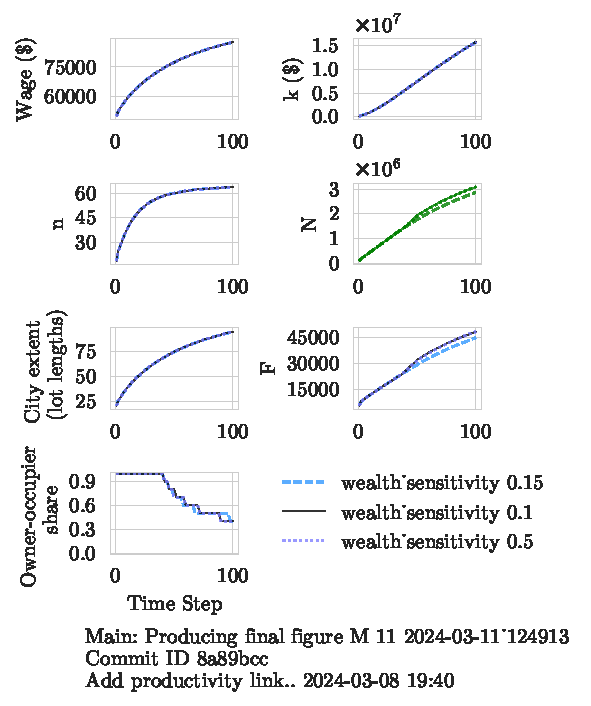
\includegraphics[width=.52\textwidth, trim={.3cm 1.4cm .8cm 0},clip]{fig/wealth_sensitivity-124913.pdf}}; 

\node[inner sep=0pt] (link) at (8.3,0)
{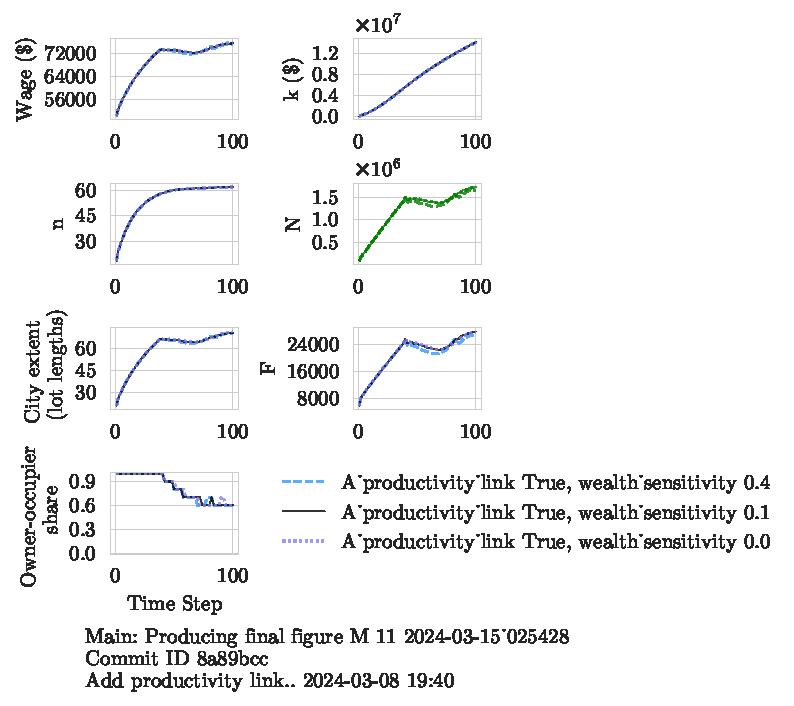
\includegraphics[width=.5\textwidth, trim={.1cm 1.4cm 4.75cm 0},clip]{fig/With-productivity_link-wealth_sensitivity-025428.pdf}};
\draw[color=white, fill=white] (8.5,-2.5) rectangle (12.6,-4);

\end{tikzpicture}
\caption[Wealth sensitivity parameter with and without linkage]{Comparing the effect of the wealth sensitivity parameter with and without a productivity linkage, with wealth sensitivity parameter values of 0.1, 0.15, and 0.5. The wealth sensitivity parameter controls the wealth required for accessing a mortgage, and its effect is illustrated in Figure~\ref{fig:Wealth-based} in the model chapter.}
\label{fig:Productivity_link_W-WO-wealth}
\end{figure}
With or without productivity links, a restrictive mortgage regime slightly reduces the labour supply and city population. It has no noticeable effect on the ownership ratio. In the presence of a productivity linkage, the population is more variable and lower. %is cut roughly in half. 
Wages are lower, consistent with lower rents in a smaller city. With low growth, property speculation is not profitable and investors do not enter the market. The ownership ratio is, therefore, higher not because there are more owners, but because there are fewer investment properties. 
%In the presence of a productivity linkage, the population is more variable and is cut roughly in half. Wages are lower, consistent with lower rents.
% \begin{figure}[h!bt]
%     \centering
%     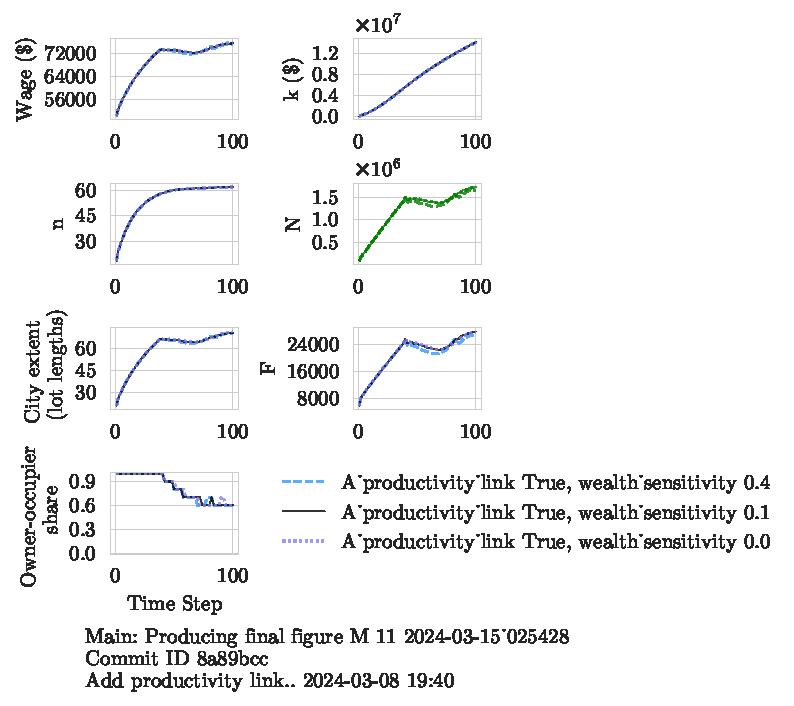
\includegraphics[scale=1, trim={0 1.4cm 0 0},clip]{fig/With-productivity_link-wealth_sensitivity-025428.pdf}
%     \caption[The effect of the wealth sensitivity parameter with a productivity linkage]{The effect of the wealth sensitivity parameter with a productivity linkage. The figure illustrates the effect of the parameter on seven policy variables over time, with parameter values of 0.15, 0.1, and 0.5. The wealth sensitivity parameter controls the wealth required for accessing a mortgage. {\color{red} Figure~\ref{} in Chapter~\ref{chapter-model} on the model illustrates the effect of the parameter on the maximum mortgage available to borrowers with different asset levels.}}
%     \label{fig:Productivity_link_and_wealth_sensitivity_ownership_trajectory}
% \end{figure}
% \begin{figure}[h!tb] 
%     \centering
%     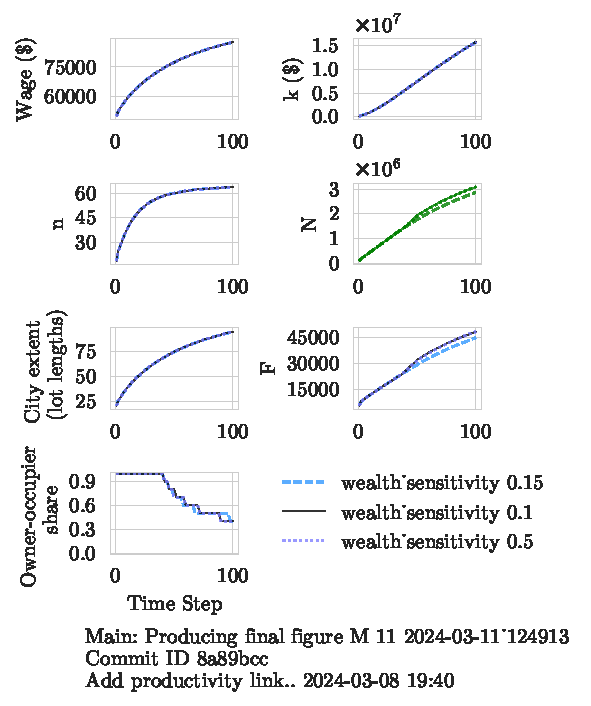
\includegraphics[scale=.75, trim={0 1.4cm .8cm 0},clip]{fig/wealth_sensitivity-124913.pdf} 
%     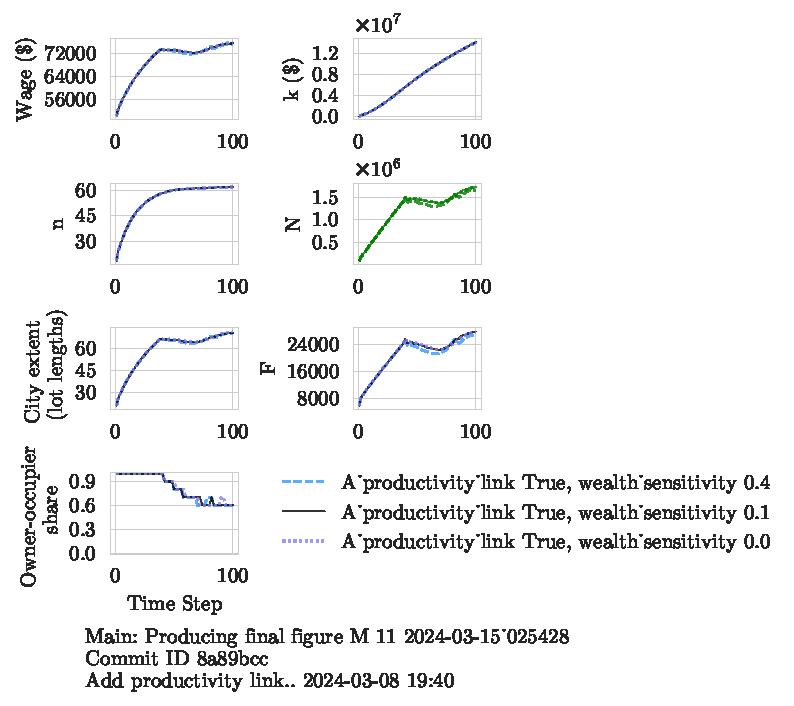
\includegraphics[scale=.75, trim={0 1.4cm 4.75cm 0},clip]{fig/With-productivity_link-wealth_sensitivity-025428.pdf} 
%     \caption[The effect of the wealth sensitivity parameter with and without a productivity linkage]{The effect of the wealth sensitivity parameter with and without a productivity linkage. The figure illustrates the effect of the parameter on seven policy variables over time, with parameter values of 0.1, 0.15, and 0.5, comparing a productivity linkage and no productivity linkage. The wealth sensitivity parameter controls the wealth required for accessing a mortgage. {\color{red} Figure~\ref{} in Chapter~\ref{chapter-model} on the model illustrates the effect of the parameter on the maximum mortgage available to borrowers with different asset levels.}}
%     \label{fig:Productivity_link_W-WO-wealth}
% \end{figure}

\newpage
\subsection{The property tax rate  with linkage}
% {\color{red} Usually you say what this figure shows first?? Then the results}
A high annual tax rate on properties 
% The effect of the property tax on the ownership share in the presence of a productivity link is minimal. 
Both high and very low property tax rates appear to decrease the ownership ratio and reduce the wage and city size. % This observation provides more evidence that the effect of public sector policies may differ in the presence of a productivity link, and that merits further investigation. % of this unrecognized variable % should be on the research agenda of urban theorists and policy-makers.
\begin{figure}[h!tb]   
    \centering
    \begin{tikzpicture}
\node[inner sep=.5pt] (plain) at (-2,0)
    {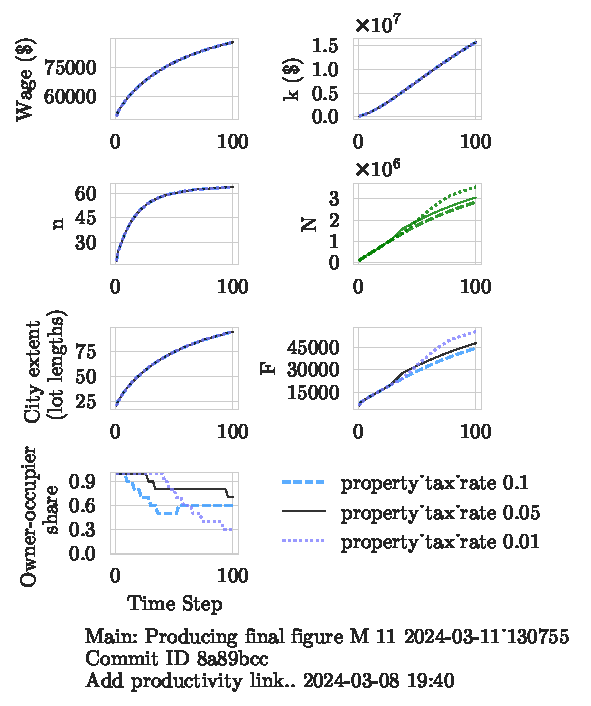
\includegraphics[height=10cm,%width=.5\textwidth,
    trim={.2cm 1.4cm .1cm 0},clip]{fig/property_tax_rate-Main-130755.pdf}}; 

\node[inner sep=0pt] (link) at (6,0)
    {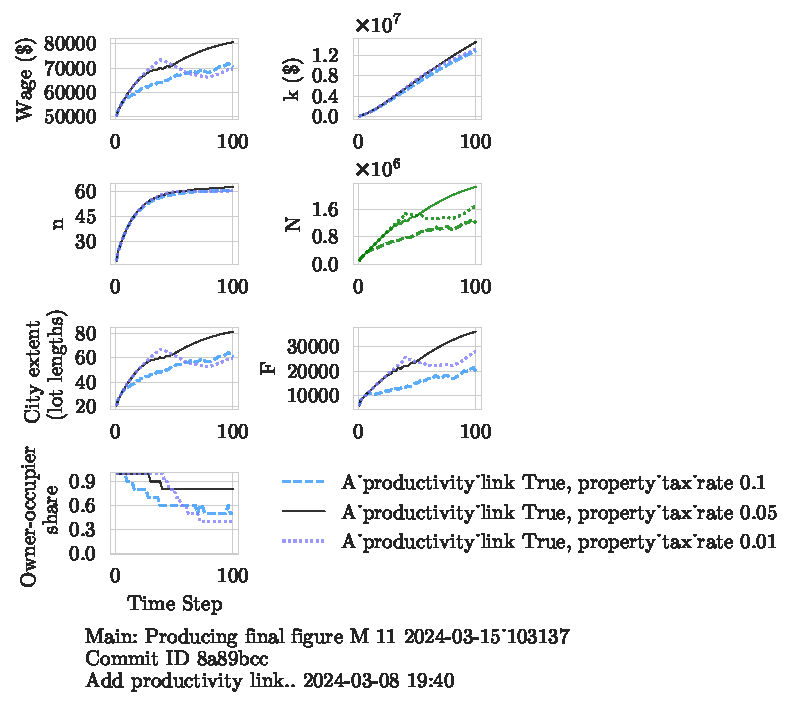
\includegraphics[height=10cm,%width=.5\textwidth, 
    trim={0cm 1.4cm 5.cm 0},clip]{fig/With-productivity_link-property_tax-103137.pdf}};
    
\draw[color=white, fill=white] (6,-2.3) rectangle (10.2,-4.5);
\end{tikzpicture}
       \caption[Varying the property tax rate with and without  linkage]{Comparing the effect of varying the property tax rate with and without a productivity linkage. Illustrates the effect on seven policy variables over time, with rates between 1\% and 17\%.}
    \label{fig:Productivity_link_W-WO-property_tax}
\end{figure}
% \subsubsection{The property tax rate}
With a productivity link, differences in the property tax rate have a much more dramatic effect on wages and urban size. The variable effect is clear from the spread of the lines on the right panel of Figure~\ref{fig:Productivity_link_W-WO-property_tax}.   % of this unrecognized variable


% {\color{red} NOT SURE WHERE THIS FITS? Speculative cycles are not strong for values in the typical range of real property taxes.}

% 'property_tax_rate': [0.1, 0.05, .01] k doing}
% \begin{figure}[h!tb]
%     \centering
%     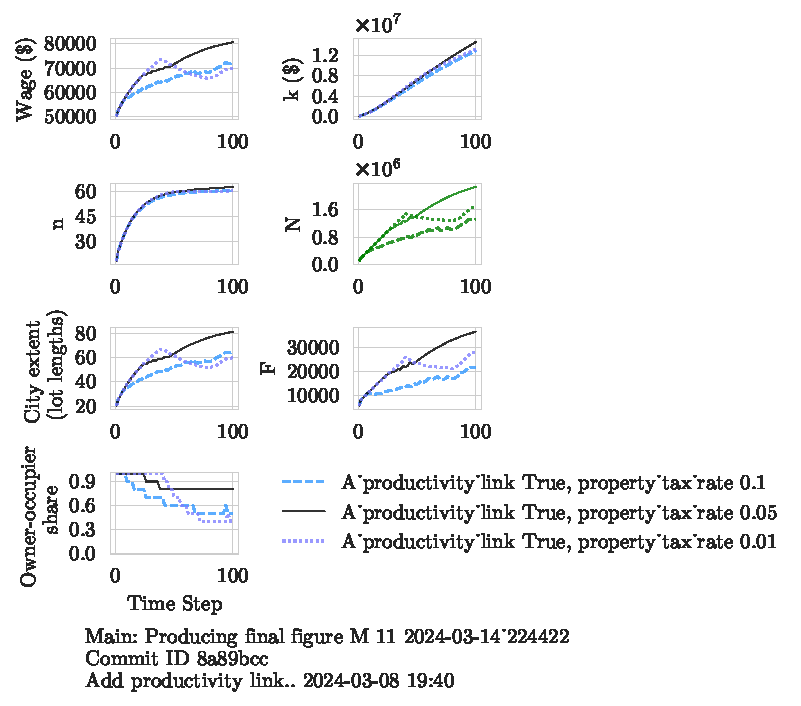
\includegraphics[scale=.8, trim={0 1.4cm 0 0},clip]{fig/With-productivity_link-property_tax-224422.pdf}%  Alternative: 103137.pdf}
%     \caption{The effect of property tax rates in the presence of productivity impacts}
%     \label{fig:Productivity_link_and_property_tax_ownership_trajectory}
% \end{figure}
% \begin{figure}[h!tb] 
%     \centering
%     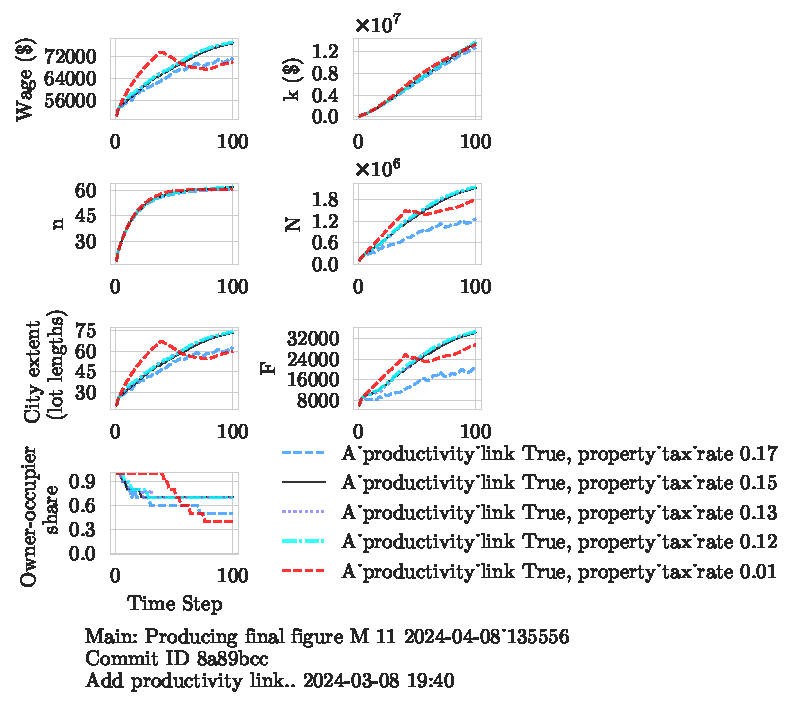
\includegraphics[scale=1, trim={0 1.4cm 0 0},clip]{fig/link-property_tax_135556.pdf}  %224422.pdf}%  Alternative:
%     \caption[The effect of varying the property tax rate with a productivity linkage]{The effect of varying the property tax rate with a productivity linkage. Illustrates the effect on seven policy variables over time, with rates between 1\% and 17\%.}
%     \label{fig:Productivity_link_and_property_tax_ownership_trajectory}
% \end{figure}
% \begin{figure}[h!tb] 
%     \centering
%     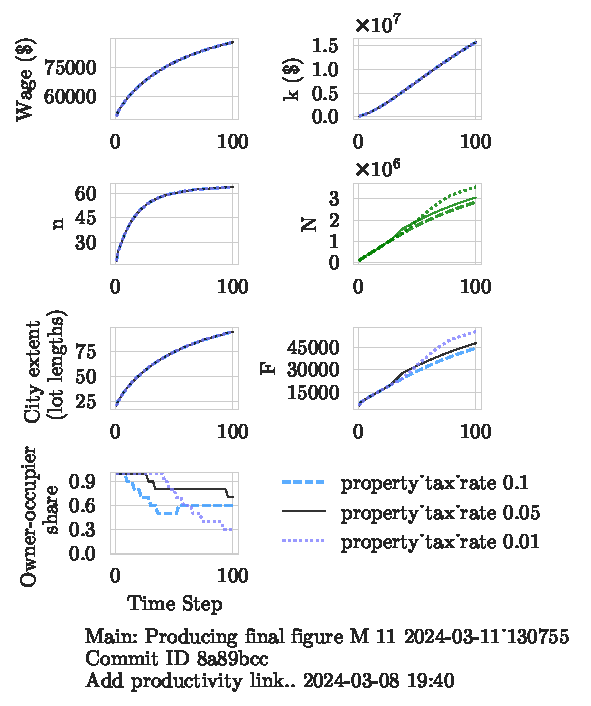
\includegraphics[scale=.75, trim={0 1.4cm .8cm 0},clip]{fig/property_tax_rate-Main-130755.pdf} 
%     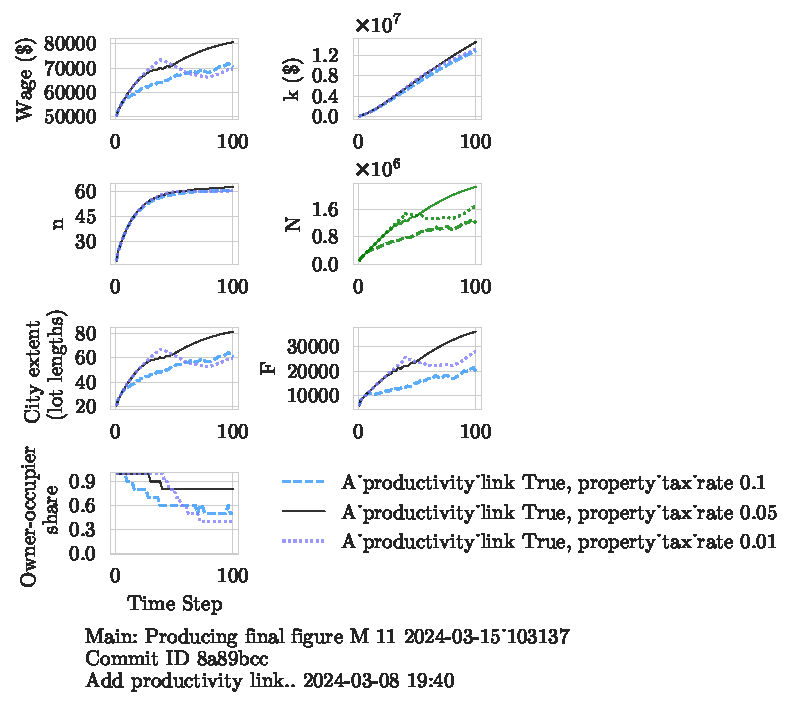
\includegraphics[scale=.75, trim={0 1.4cm 4.75cm 0},clip]{fig/With-productivity_link-property_tax-103137.pdf} 
%     \caption[The effect of varying the property tax rate with and without a productivity linkage]{The effect of varying the property tax rate with and without a productivity linkage. Illustrates the effect on seven policy variables over time, with rates between 1\% and 17\%, comparing a productivity linkage and no productivity linkage.}
%     \label{fig:Productivity_link_W-WO-property_tax}
% \end{figure}

\newpage
\section{Transitory policy shocks}

% Policies are not set at the beginning of a city's life and retained forever. They are introduced and adjusted at various points in the history of a city. %, as we did in all the illustrations above.
This section explores the effect of a change in policy using our model and illustrates that policy shocks appear to drive cyclic behaviour with the linkage.

\subsection{A temporary surge of speculation}
After 50 years of growth with a capital gains tax on investors of 100\%, we reduce the capital gains to zero for 25 years, then return the tax level to 100\%, with the productivity linkage. The blue dashed line shows the case with the capital gains tax held at 100\%. There is no property speculation because no capital gains are available to investors.
\begin{figure}[h!tb]   
    \centering
    \begin{tikzpicture}
%\draw[step=1.0,black,thin] (-4,-5) grid (4,5);
\node[inner sep=.5pt] (plain) at (0,0)
    {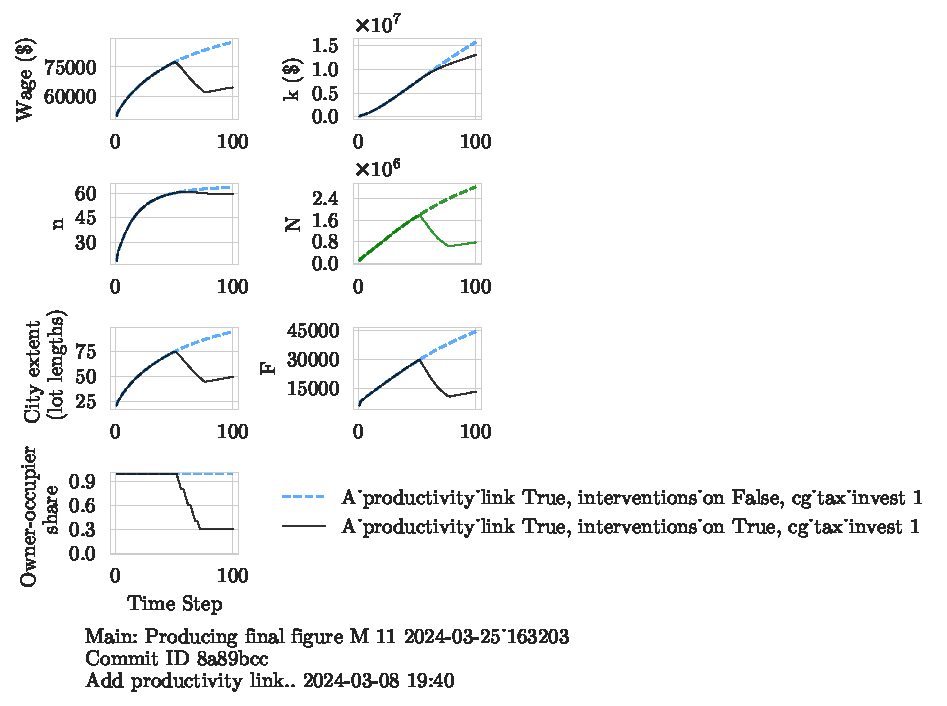
\includegraphics[height=10cm,%width=.5\textwidth,
    trim={.2cm 1.4cm 7.5cm 0},clip]{fig/interventions_on-cg_tax_invest-163203.pdf}}; 

% \node[inner sep=0pt] (link) at (6,0)
%     {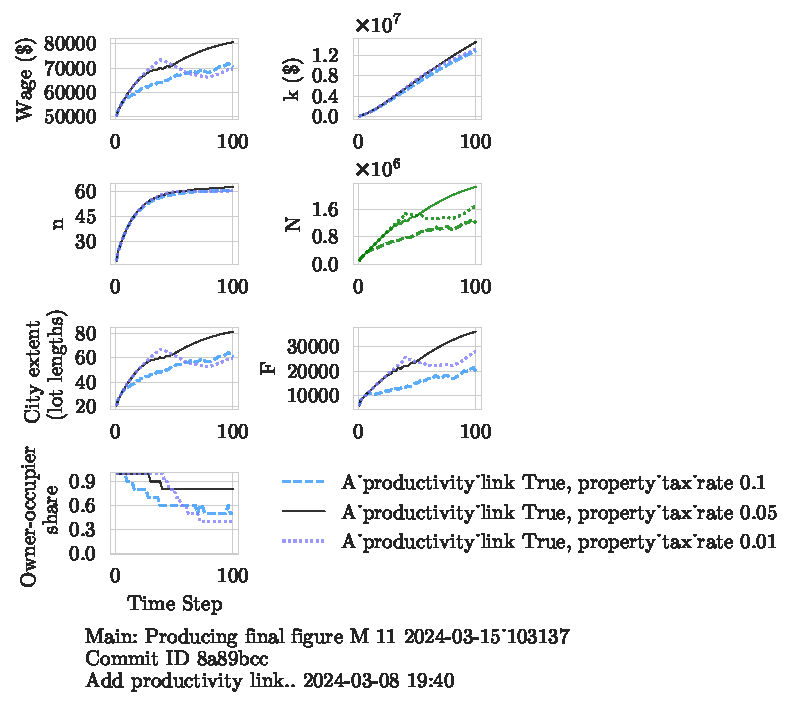
\includegraphics[height=10cm,%width=.5\textwidth, 
%     trim={0cm 1.4cm 5.cm 0},clip]{fig/With-productivity_link-property_tax-103137.pdf}};

\begin{scope}[shift={(1.2,-4.07)}]
\draw[color=white, fill=white, fill= white] (0,0) rectangle (2.8,1.5);   %, fill=white]
\node at (1.6,1.05)[align=left, scale=01.2]{\tiny 100\% capital gains tax};
\node at (1.4,.58)[align=left,  scale=01.2]{\tiny temporary zero  tax};
\end{scope}

\end{tikzpicture}
      \caption[Temporarily reducing the capital gains tax for investors from 100\% ]{The effect of temporarily reducing the capital gains tax for investors from 100\% to zero for 25 years, with the productivity linkage. The black line shows the case with the policy shock. The blue dashed line shows the reference case in which the original 100\% capital gains tax is maintained.}
\label{fig:cgtax_setback}
\end{figure}
% \begin{figure}[h!tb] 
% \centering
% % \raggedleft
% % \hspace{5cm}
% \includegraphics[scale=0.9, trim={0 1.4cm 7cm 0},clip]{fig/interventions_on-cg_tax_invest-163203.pdf}  %224422.pdf}%  Alternative:
% \caption[The effect of temporarily reducing the capital gains tax for investors from 100\% to zero for 25 years]{The effect of temporarily reducing the capital gains tax for investors from 100\% to zero for 25 years, with the productivity linkage.}
% \label{fig:cgtax_setback}
% \end{figure}
The solid black line shows that, following the drop in the investor capital gains tax,  the owner-occupier share of housing falls to 30\%, meaning 70\% of the city housing stock is financialized. 
With the intervention, there is also a steady decline in wages, some reduction in firm size and capital stock, a two-thirds reduction in population and number of firms, and a one-third reduction in city diameter, over the 25 periods. At the end of that period, the city has declined to a level approximately where it was at approximately thirty-years periods before the policy change. %The slow growth is associated with the decline in home-ownership arising from the change in the capital gains tax on speculation. 
% Reversing the policy, the city returns to a growth rate that is lower than when the policy was implemented, suggesting the possibility that the urban system may display hysteresis, not returning to its original path after a shock. % Even after 300 periods (not shown) it does not return to its original path.
% The homeownership ratio is a state variable of the system that lacks a returning force.
% In this dramatic example, we have used a policy variable that we know can have a powerful effect and have assumed a strong productivity linkage. % Despite the exaggerated effect, this example demonstrates that the model could be used to examine policy innovations. 
% not be resilient in the sense of 


% \subsection{Variant with 300-year time horizon, different initial level of the capital gains tax}
% A 100\% capital gains tax is a useful reference case, but it is not realistic, so we consider an initial capital gains tax on investors of 15\%, closer to the actual case. After 50 years of growth with a 15\% rate we reduce the capital gains for investors to zero for 25 years as we did in the previous example. After 50 years we change the tax level to 100\%.  
% \begin{figure}[h!tb] 
% \centering
% % \raggedleft
% % \hspace{5cm}
% \includegraphics[scale=0.9, trim={0 1.4cm 3cm 0},clip]{fig/Link-CGI-15-0-100-300-years.pdf}%  Alternative:
% \caption[The effect of temporarily reducing the capital gains tax for investors from 15\% to zero for 25 years]{The effect of temporarily reducing the capital gains tax for investors from 15\% to zero for 25 years and then to 100\%, with the productivity linkage.}
% \label{fig:cgtax_setback}
% \end{figure}
% In this case the blue line represents the path of the economy with a 15\% Capital gains tax Following the drop in the investor capital gains tax. The city is smaller and investors own more of the housing.  
% The solid black line in Figure~\ref{fig:cgtax_setback} shows the effect of dropping the tax to zero for 50 years then raising it to 100\%.

% \subsection{Encouraging speculation, then reversing  policy}


\newpage
\subsection{Variant with 300-year time horizon, different initial level of the capital gains tax}
To explore a slightly more realistic situation, we consider an initial capital gains tax on investors of 15\%, rather than 100\%. After 50 years of growth with a 15\% rate we reduce the capital gains for investors to zero for 25 years as we did in the previous example. After 50 years we return the tax level to 100\% to remove the effect of any further speculative investment. 
\begin{figure}[h!tb]   
    \centering
    \begin{tikzpicture}

\node[inner sep=.5pt] (plain) at (0,0)
    {\includegraphics[height=10cm,%width=.5\textwidth,
    trim={.2cm 1.4cm 5.5cm 0},clip]{fig/Link-CGI-15-0-100-300-years.pdf}}; 

% \node[inner sep=0pt] (link) at (6,0)
%     {\includegraphics[height=10cm,%width=.5\textwidth, 
%     trim={0cm 1.4cm 5.cm 0},clip]{fig/With-productivity_link-property_tax-103137.pdf}};

%\draw[step=.5, thin, gray!30] (-5,-5) grid (5,5);

\begin{scope}[shift={(1.,-4.07)}]
\draw[color=white, fill=white, fill= white] (0,0) rectangle (2.8,1.5);   %, fill=white]
\node at (1.6,1.05)[align=left, scale=01.2]{\tiny 15\% capital gains tax};
\node at (2.2,.58)[align=left,  scale=01.2]{\tiny temporary zero then 100\% tax};
\end{scope}

\end{tikzpicture}
      \caption[Temporarily reducing the capital gains tax for investors: 300 years run]{The effect of temporarily reducing the capital gains tax for investors from 100\% to zero for 25 years, with the productivity linkage. The black line shows the case with the policy shock. The blue dashed line shows the reference case in which the original 15\% capital gains tax is maintained.}
\label{fig:cgtax_setback2}
\end{figure}
% \begin{figure}[h!tb] 
% \centering
% % \raggedleft
% % \hspace{5cm}
% \includegraphics[scale=0.9, trim={0 1.4cm 3cm 0},clip]{fig/Link-CGI-15-0-100-300-years.pdf}%  Alternative:
% \caption[The effect of temporarily reducing the capital gains tax for investors from 15\% to zero for 25 years]{The effect of temporarily reducing the capital gains tax for investors from 15\% to zero for 25 years, with the productivity linkage.}
% \label{fig:cgtax_setback}
% \end{figure}
% % 
In this case, the dashed blue line represents the path of the economy with a 15\% capital gains tax following the drop in the investor capital gains tax. % In this case, 
With a sustained capital gains tax on speculation of only 15\%, the city is smaller and investors own more of the housing. About half of the housing stock is captured by the financial sector. 
Growth is slower growth than in the case that began with 100\% capital gains tax. %, and a series of speculative waves occurs. % as shown by blue dashed lines in the upper panels.  
The solid black line in Figure~\ref{fig:cgtax_setback2} shows the %case described in the section above, in which the 
effect of dropping the tax to zero for 50 years then raising it to 100\%. Again, the trajectory displays a sharp drop and a slow return.  


% \begin{figure}[h!tb] 
% \centering
% % \raggedleft
% % \hspace{5cm}
% \includegraphics[scale=0.9, trim={0 1.4cm 5cm 0},clip]{fig/link-interv_CGI-B-pt15_0-50_1-75230845.pdf}%  Alternative:
% \caption[The effect of temporarily reducing the capital gains tax for investors from 15\% to zero and then raising it to 100\%]{The effect of temporarily reducing the capital gains tax for investors from 15\% to zero and then raising it to 100\%, with the productivity linkage.}
% \label{fig:cgtax_setback2}
% \end{figure}




% link-interv_CGI-B-pt15_0-50_1-75230845.
%{\color{red} ADD A SUMMARY SAYING THAT THIS SUGGESTS THAT EFFECTS OF POLICY DEPENDS ON WHERE YOU ARE IN A SYSTEM... explain what is suggests }

\section{Summary}


We set out to explore the two propositions:
\begin{enumerate} 
\item Financialization of the housing market will result in the tenantization of the urban middle class as financial capital acquires more of the housing stock. % vs decline of the urban middle class
\item Financialization of the housing market could result in reduced growth of urban productivity as the flow of rents is diverted from real investment to the financial sector.
\end{enumerate} 
In this chapter, we have thus explored two things. First, what policy interventions might affect the basic financialization ownership result, reducing or increasing the rate at which financialized actors take over the urban housing market and their penetration of the market? Second, what would the effect be if there were a feedback linkage between financialization and productivity? 


We presented 84 outputs from experiments about policy actions in our model, examining the effect of seven policy interventions on seven economic variables. Forty-two of the outputs explore the effects without a linkage between financialization and productivity, and forty-two explore the effect with the linkage added. % with what the effects of policy are when there is a link between financialization and urban productivity. 
% We believe we are the first to explore this question systematically with a formal simulation model.
We did not demonstrate that the link exists, although we laid out seven channels through which a linkage might act in Chapter~\ref{chapter-tramsmission}, and the discussion in that chapter strongly suggessts that there may be such a linkage. % This is important because we have not found other work that explore the effect of a link between financialization and urban productivity using simulation models. 
The results in this chapter suggest that the linkage, if it exists, would have a powerful impact on the city, and thus that further research on the linkages between productivity and financialization could play a powerful role in improving our understanding of the way the urban economy is evolving. %and suggest that further research on linkages and their effects could improve % how to implement them with models like ours  

More generally, several observations may be drawn from our results: 
\begin{enumerate}
\item In the absence of linkages between the housing market and the production sector, of the policy tools we consider, only density and transportation have a substantial effect on ownership or the other economic variables. % {\color{red} ON WHAT??  economic variables ??like ???? MAYBE MAKE THIS INTO A LIST? }

\item In the presence of linkages, policy tools have much more dramatic effects. % This is potentially a very important result. 
The presence of linkages seems to make the city vulnerable, not just to static effects, but to cycles of speculation that could induce boom-bust cycles. 

%we see population effects but no effect on firm variables wage, capital stock or workforce. This is because we force the number of firms to accommodate increases in population. Different assumptions would have allowed growth in both firm size and number, but we were interested in the evolution of population, productivity and ownership rather than the details of the production sector. 

\item A capital gains tax on speculative investment in housing has a powerful and positive effect on economic variables, both with and without a productivity linkage. Without the linkage, a higher tax on investors increases owner-occupancy. With a productivity linkage, there are also effects on economic markers, as reducing the capital gains tax reduces the size of the city and wages. 

\item Increasing the capital gains tax on owner-occupiers above the level of the capital gains tax on investors has a powerful negative effect on population and wages.

\item The cost of capital has surprisingly little effect on any variables in either case.

\item Transportation cost has a strong effect on city growth rate and size, as expected. It also decreases the home-ownership ratio, likely because of the attractiveness of a more rapidly growing city to investors. Warranting further investigation is that low transportation costs with financial system spillovers appear to induce something like cyclical behaviour.

\item Increasing density increases the population but does not affect wages, city extent, or ownership ratios, as expected.

\item A more restrictive mortgage market does not affect the production sector, city size or ownership ratios with or without the linkage.

\item Increasing property taxes has a mixed effect on the number of owner-occupiers and city size when there is no linkage to financialization, but depresses wages, population and city size when there is a linkage. 
\end{enumerate}
%$${\color{red} ADD A SUMMARY saying that this provides useful information about .... and suggests that WHICH in particular would be useful to study further. AND say that also studying shifts mid=trajectory would be useful as the shock thing suggests.


While these results do not allow us to make claims about the world outside the model, they do provide indications of areas that would be useful to explore further. 